\documentclass[12pt,a4paper]{article}
\usepackage[utf8]{inputenc}
\usepackage[T1]{fontenc}
\usepackage{mathptmx}
\usepackage[margin=2.5cm]{geometry}
\usepackage{setspace}
\singlespacing
\usepackage{graphicx}
\usepackage{amsmath,amssymb,amsfonts}
\usepackage{booktabs}
\usepackage{array}
\usepackage{multirow}
\usepackage{longtable}
\usepackage{float}
\usepackage{caption}
\usepackage{subcaption}
\usepackage{hyperref}
\usepackage{xcolor}
\usepackage{enumitem}
\usepackage{fancyhdr}
\usepackage{titlesec}
\usepackage{tocloft}
\usepackage{appendix}
\usepackage{pdflscape}
\usepackage{tikz}

\setlength{\parindent}{0pt}
\usetikzlibrary{shapes,arrows,positioning}
\hypersetup{colorlinks=true,linkcolor=blue,filecolor=magenta,urlcolor=cyan,citecolor=blue}
\pagestyle{fancy}
\fancyhf{}
\fancyfoot[C]{\thepage}
\renewcommand{\headrulewidth}{0pt}
\titleformat{\section}{\Large\bfseries}{\thesection}{1em}{}
\titleformat{\subsection}{\large\bfseries}{\thesubsection}{1em}{}
\titleformat{\subsubsection}{\normalsize\bfseries}{\thesubsubsection}{1em}{}
\setcounter{tocdepth}{3}

\begin{document}
\graphicspath{{figures/}}

% ============================================

% COVER PAGE

% ============================================

\begin{titlepage}

% Left side logo
\begin{tikzpicture}[remember picture,overlay]
  \node[anchor=north west] at ([xshift=1.5cm,yshift=-2cm]current page.north west) {
    
\includegraphics[width=2.5cm]{tbs_logo.png}
  };
\end{tikzpicture}

\centering

\vspace*{1cm}

{\Large\bfseries\color{red!70!black} TBS}\\[0.2cm]

{\small\color{red!70!black} EDUCATION}\\[0.5cm]

{\footnotesize INSPIRING EDUCATION INSPIRING LIFE}

\vspace{2cm}

{\large MASTER OF SCIENCE}\\[0.3cm]

{\large ACADEMIC YEAR 2024/2025}

\vspace{3cm}

{\Huge\bfseries MASTER DISSERTATION}

\vspace{1.5cm}

{\LARGE\bfseries Deep Learning Framework for Heston Model Calibration}

\vspace{0.5cm}

{\large\itshape Neural Network Surrogate Models for Accelerated Option Pricing Model Calibration}

\vspace{3cm}

\begin{tabular}{rl}
\textbf{Author:} & Joris Marvezy \\[0.3cm]
\textbf{Program:} & MSc Equity Research and Investment Management \\[0.3cm]
\textbf{Academic Supervisor:} & M. Mamonov \\[0.3cm]
\textbf{Submission Date:} & November 30, 2025 \\
\end{tabular}

\vfill

{\footnotesize AACSB $\cdot$ EQUIS $\cdot$ AMBA}

\end{titlepage}  
  

% ============================================

% TABLE OF CONTENTS

% ============================================

\newpage

\tableofcontents

% ============================================

% LIST OF FIGURES

% ============================================

\newpage

\listoffigures

\addcontentsline{toc}{section}{List of Figures}

% ============================================

% LIST OF TABLES

% ============================================

\listoftables

\addcontentsline{toc}{section}{List of Tables}

% ============================================

% EXECUTIVE SUMMARY

% ============================================

\newpage

\section*{Executive Summary}

\addcontentsline{toc}{section}{Executive Summary}

This master dissertation develops and empirically evaluates a deep learning framework for calibrating the Heston stochastic volatility model to real market option prices. The research addresses a fundamental challenge in quantitative finance: balancing computational efficiency with pricing accuracy in model calibration.

\textbf{Context and Motivation.} Option pricing model calibration is computationally intensive, requiring hundreds of numerical pricing evaluations per optimization. For financial institutions managing large portfolios, traditional calibration methods create operational bottlenecks that limit recalibration frequency and responsiveness to market changes.

\textbf{Research Approach.} The framework develops a neural network surrogate model that approximates the Heston pricing function, enabling fast inference during calibration. The framework incorporates security-specific parameter ranges derived from historical volatility statistics, importance sampling for training data generation, and a hybrid methodology combining neural network speed with traditional accuracy guarantees. Empirical evaluation spans three securities (QQQ, SPY, TSLA) representing diverse volatility regimes, comprising 288 option contracts.\\[0.5cm]

\textbf{Key Findings.}

\begin{itemize}[noitemsep]

\item \textbf{Computational Efficiency}: Average speedup of 2.27$\times$ (range: 0.81$\times$ to 3.59$\times$), with best performance for moderate-volatility securities with large option sets.

\item \textbf{Pricing Accuracy}: Systematic accuracy degradation of 6.9--160\% (RMSE) depending on security characteristics, with neural network consistently underpricing options.

\item \textbf{Statistical Robustness}: All differences statistically significant at $\alpha = 0.01$ after multiple comparison corrections; effect sizes range from small (Cohen's $d = 0.33$) to medium ($d = 0.54$).

\item \textbf{Context Dependence}: Performance varies substantially by security: QQQ shows excellent results (6.9\% RMSE increase, 3.59$\times$ speedup), while TSLA shows challenging performance (160\% RMSE increase, no speedup).

\item \textbf{Hybrid Recommendation}: The optimal deployment strategy employs neural network initialization followed by traditional FFT refinement, achieving balanced speedup (2.4$\times$) with acceptable accuracy degradation (8.3\% RMSE increase).

\end{itemize}

\textbf{Practical Implications.} For a 100-security portfolio with daily recalibration, the framework saves approximately 16 hours of computation annually. The hybrid approach provides optimal balance for production systems requiring both speed and accuracy guarantees.

% ============================================

% ACKNOWLEDGEMENTS

% ============================================

\newpage

\section*{Acknowledgements}

\addcontentsline{toc}{section}{Acknowledgements}

I would like to express my sincere gratitude to all those who have helped in one way or another in making this work a success.

I would like to extend my appreciation to TBS Education for providing the academic framework and resources that made this research possible. Special thanks, especially, to the corporate staff, whose support and assistance have been particularly relevant to the success of this work.

I extend special thanks to three YouTube creators who have helped me greatly in understanding the concepts of neural networks and deep learning, applied to finance:

\begin{itemize}[noitemsep]

\item \textbf{3Blue1Brown}: For his videos on neural networks, deep learning and all the mathematics behind it, available on YouTube.

\item \textbf{QuantPy}: For his videos on quantitative finance and the application of the Heston framework to real market data, available on YouTube.

\item \textbf{Roman Paolucci}: For his videos on neural networks, deep learning and finance, available on YouTube.

\end{itemize}

To my family and friends, thank you for your unwavering support and understanding during this research process.

% ============================================

% SECTION 1: INTRODUCTION

% ============================================

\newpage

\section{Introduction}

\label{sec:introduction}

\subsection{Background and Context}

Derivatives, particularly options, have become fundamental instruments in modern financial markets. Options provide investors with flexible strategies for risk management, speculation, and portfolio optimization. The global options market has experienced exponential growth, with daily trading volumes exceeding hundreds of billions of dollars across equity, index, and commodity options.

Accurate option pricing is essential for market making (quoting bid-ask spreads reflecting fair value), risk management (computing Greeks for hedging strategies), regulatory compliance (demonstrating robust pricing models for capital requirements), and trading strategies (identifying mispricings and arbitrage opportunities). The complexity of option pricing arises from the need to model the underlying asset's future price evolution, particularly capturing volatility dynamics, one of the most challenging aspects of financial modeling.

\subsection{The Volatility Challenge}

Volatility, the measure of price uncertainty, is not directly observable in financial markets (we can only infer its value from observable prices). This presents several fundamental challenges:

\textbf{Volatility Clustering}: Financial markets exhibit volatility clustering, meaning that periods of high volatility tend to be followed by other periods of high volatility, contradicting constant volatility assumptions.

\textbf{Volatility Smiles and Skews}: Market-implied volatilities vary systematically with strike price and maturity, creating characteristic smile or skew patterns inconsistent with the Black-Scholes constant volatility model.

\textbf{Leverage Effect}: A negative correlation exists between asset returns and volatility changes: when prices fall, volatility tends to increase. This observation, known as the leverage effect, manifests as the volatility skew in equity options markets.

\textbf{Mean Reversion}: Volatility exhibits mean-reverting behavior, reverting to long-term average levels over time.

These stylized facts necessitate stochastic volatility models such as Heston \cite{Heston1993}, which treats volatility as a random process rather than as a constant value, as assumed in the Black-Scholes \cite{BlackScholes1973} and Merton \cite{Merton1973} framework.

\subsection{The Challenge of Model Calibration}

Model calibration (estimating parameters such that theoretical prices match observed market prices) faces significant computational challenges. Stochastic volatility models require numerical methods (FFT, numerical integration) taking milliseconds to seconds per option. Calibration requires 50--500 iterations, each pricing all options in the calibration set. Financial institutions must calibrate models for hundreds of securities simultaneously. For a portfolio of 100 securities with 200 options each, even 10-second calibration per security requires 555 hours annually.\\[0.5cm]

\subsection{The Rise of Machine Learning in Quantitative Finance}

Neural networks, as universal function approximators, can learn the mapping from model parameters to option prices, serving as fast surrogate models. Once trained, neural networks can evaluate thousands of option prices in milliseconds through highly optimized matrix operations, offering orders of magnitude speedup over traditional numerical methods.

\subsection{Problem Statement and Research Questions}

The core research problem is: \textit{Can neural network surrogate models accelerate Heston stochastic volatility model calibration to real market option prices while maintaining acceptable accuracy, and what are the quantitative trade-offs between computational speed and pricing accuracy?}\\[0.05cm]

This dissertation addresses four key research questions:\\[0.05cm]

1. What is the quantitative speedup achieved through neural network surrogate calibration compared to traditional FFT-based methods?\\[0.05cm]

2. What is the accuracy degradation when using neural network surrogates, and how does it vary across securities?\\[0.05cm]

3. How does neural network calibration perform across different securities, volatility regimes, and market conditions?\\[0.05cm]

4. Under what conditions should practitioners prefer neural network calibration over traditional methods?


% ============================================

% SECTION 2: LITERATURE REVIEW

% ============================================

\newpage

\section{Literature Review}

\label{sec:literature}

\subsection{Classical Option Pricing and the Black-Scholes-Merton Paradigm}

\subsubsection{The Foundational Framework}

Black and Scholes \cite{BlackScholes1973} and Merton \cite{Merton1973} revolutionized financial economics by deriving the celebrated closed-form solution for European option prices. The Black-Scholes formula:

\begin{equation}
C_{\text{BS}} = S_t N(d_1) - K e^{-r\tau} N(d_2),
\end{equation}

where $d_1 = \frac{\ln(S_t/K) + (r + \sigma^2/2)\tau}{\sigma\sqrt{\tau}}$ and $d_2 = d_1 - \sigma\sqrt{\tau}$, established the no-arbitrage pricing paradigm that remains foundational to modern derivatives valuation. The framework's elegance lies in reducing option valuation to five observable or estimable quantities: spot price $S_t$, strike $K$, risk-free rate $r$, time to maturity $\tau$, and volatility $\sigma$. This work, recognized with the 1997 Nobel Prize in Economics, transformed derivatives from exotic financial instruments into standardized, theoretically-grounded products.

However, the Black-Scholes model rests on restrictive assumptions: constant volatility, no transaction costs, frictionless markets, log-normal price distributions, and continuous trading. These assumptions, while enabling analytical tractability, prove unrealistic in practice. Market frictions exist, volatility varies dynamically, and empirical return distributions exhibit fat tails. Recognizing these limitations motivates substantial post-Black-Scholes research.

\subsubsection{Empirical Deviations: The Volatility Smile and Term Structure}

Rubinstein \cite{Rubinstein1985} conducted the most comprehensive early empirical examination of Black-Scholes predictions using CBOE data on 30 active option classes from November 1981 to March 1985. His analysis of 2.5 million option quotes revealed systematic deviations from Black-Scholes predictions, particularly a pronounced ``volatility smile'': out-of-the-money puts exhibited 2-4 percentage points higher implied volatility than at-the-money options, with the pattern intensifying following the 1987 stock market crash. This smile pattern, characterized by higher implied volatilities at extreme moneyness, directly contradicts the Black-Scholes constant volatility assumption and cannot be reconciled within the framework.

Subsequent research quantified volatility dynamics' importance. Lamoureux and Lastrapes \cite{Lamoureux1993} analyzed implied volatility time series for S\&P 500 options (1983-1991), documenting strong autocorrelation with half-lives of volatility shocks measured in weeks to months, contradicting any constant volatility model. Their GARCH-M specifications demonstrated that volatility fluctuations exhibit mean reversion rather than random walks, with long-memory properties suggesting that current volatility conveys information about future volatility.

Black \cite{Black1976} pioneered documentation of the leverage effect, the empirical observation that stock returns exhibit negative correlation with volatility changes. As equity prices fall, uncertainty about future cash flows increases, driving volatility up. This asymmetry consisting in positive returns associated with volatility decreases and negative returns with volatility increases, becomes quantitatively significant, with leverage correlations reaching -0.3 to -0.7 in equity markets. This stylized fact motivates models incorporating correlated price-volatility dynamics.

\subsection{Stochastic Volatility Models: Theoretical Development}

\subsubsection{Early Attempts: Hull-White and Stein-Stein Models}

Hull and White \cite{Hull1987} pioneered continuous-time stochastic volatility by permitting variance to follow its own diffusion process, enabling price and volatility to exhibit nonzero correlation. Their model specified variance dynamics:

\begin{equation}
dV_t = \mu_V V_t \, dt + \sigma_V V_t \, dW_t^2,
\end{equation}

with correlation $\langle dW_t^1, dW_t^2 \rangle = \rho \, dt$. While capturing stylized facts like volatility clustering, the Hull-White specification limited analytical tractability, requiring numerical methods for option pricing.

Stein and Stein \cite{SteinStein1991} developed an alternative specification with absolute volatility dynamics:

\begin{equation}
d\sigma_t = \kappa(\bar{\sigma} - \sigma_t) \, dt + \sigma_V \, dW_t^2,
\end{equation}

enabling mean reversion and permitting negative volatility with positive probability, a theoretical drawback. While their framework allowed semi-closed-form solutions via Fourier transform methods, computational complexity remained prohibitive for calibration to large option sets.

\subsubsection{The Heston Breakthrough: Tractable Stochastic Volatility}

Heston \cite{Heston1993} achieved a major breakthrough through careful model specification. Under the risk-neutral measure, Heston specifies joint dynamics for asset price $S_t$ and instantaneous variance $V_t$:

\begin{align}
dS_t &= r S_t \, dt + \sqrt{V_t} S_t \, dW_t^1, \\
dV_t &= \kappa (\theta - V_t) \, dt + \sigma \sqrt{V_t} \, dW_t^2,
\end{align}

with instantaneous correlation $\langle dW_t^1, dW_t^2 \rangle = \rho \, dt$. The five parameters have clear economic interpretations: $V_0$ (initial variance), $\kappa$ (mean-reversion speed, typical range 0.5-5), $\theta$ (long-run mean variance, typically 0.01-0.04), $\sigma$ (volatility-of-volatility, typically 0.1-1.0), and $\rho$ (leverage correlation, typically -0.8 to 0). The Feller condition $2\kappa\theta \geq \sigma^2$ ensures variance remains strictly positive with probability one, preventing negative volatility which is a theoretical necessity.

Heston's crucial insight was recognizing that variance squared term, $\sigma\sqrt{V_t}$, permits the characteristic function:

\begin{equation}
\phi(u) = \exp\{C(u, \tau) + D(u, \tau) V_t + iu \ln S_t\},
\end{equation}

where $C$ and $D$ satisfy Riccati ordinary differential equations with closed-form solutions. This analytical tractability revolutionized stochastic volatility modeling, enabling Fourier-based pricing methods.

\subsubsection{Empirical Performance: Stochastic Volatility vs. Black-Scholes}

Bakshi, Cao, and Chen \cite{BakshiCaoChen1997} conducted the most comprehensive empirical performance comparison, analyzing 38,749 S\&P 500 call option observations from June 1988 to May 1991 across four models: Black-Scholes, stochastic volatility (SV), stochastic volatility with stochastic interest rates (SVSI), and stochastic volatility with jumps (SVJ). Key findings included:

1. SV reduced out-of-the-money (OTM) pricing errors by 30-50\% versus Black-Scholes.

2. Improvements were most pronounced for short-maturity options (< 60 days), where smile effects concentrate.

3. Adding stochastic interest rates (SVSI) provided marginal improvement over SV.

4. SVJ offered best static pricing but showed limited improvement for hedging applications.

5. Pricing errors increased substantially for extreme moneyness (K/S < 0.9 or > 1.1).\\[0.05cm]

Jones \cite{Jones2003} extended this analysis by demonstrating that option-implied parameters diverge substantially from historical time-series estimates, with variance risk premia of 2-4\% annualized. This finding highlighted the importance of risk-neutral calibration for pricing versus physical calibration for forecasting.

\subsection{Alternative and Advanced Stochastic Volatility Models}

\subsubsection{Jump-Diffusion Extensions}

Merton \cite{Merton1976} pioneered jump-diffusion modeling, extending asset price dynamics to include discontinuous jumps capturing sudden market shocks:

\begin{equation}
dS_t = (r - \lambda \mathbb{E}[J_t-1]) S_t \, dt + \sqrt{V_t} S_t \, dW_t + S_t \, dN_t,
\end{equation}

where $N_t$ is a Poisson process with intensity $\lambda$ and $J_t$ represents jump magnitudes. Option prices under jump-diffusion become infinite series of Black-Scholes prices evaluated at adjusted volatilities. While capturing fat tails and jump risk premia, jump-diffusion models add complexity without fully explaining smile patterns.

\subsubsection{Rough Volatility Models}

Recent research reveals that realized volatility exhibits fractal properties more extreme than Brownian motion. Gatheral, Jaisson, and Rosenbaum \cite{GatheralJaissonRosenbaum2018} analyzed Oxford-Man Institute data spanning over 3,000 daily observations, finding Hurst parameter $H \approx 0.1$ for realized volatility, far below the $H = 0.5$ expected from standard Brownian motion. This ``rough'' behavior, characterized by rapid fluctuations with slow mean reversion, motivated rough volatility models with Hölder exponent $\alpha < 0.5$. These models capture observed volatility clustering more accurately than Heston, enabling improved smile prediction. However, rough volatility's increased complexity necessitates numerical methods more sophisticated than characteristic function approaches, generally requiring Monte Carlo simulation. The tradeoff between improved accuracy and computational complexity remains unresolved in production applications.

\subsection{Numerical Methods for Efficient Option Pricing}

\subsubsection{The Fast Fourier Transform Breakthrough}

Classical option pricing methods required numerical integration or Monte Carlo simulation, with computational costs scaling poorly in option count. Carr and Madan \cite{CarrMadan1999} introduced the fast Fourier transform (FFT) method, dramatically reducing computational complexity.

Their approach leverages the Fourier relationship between option prices and characteristic functions. By introducing damping factor $\alpha = 1.5$ ensuring integrability:

\begin{equation}
\psi(v) = \frac{e^{-rT} \phi(v - i(\alpha + 1))}{(\alpha + iv)(\alpha + 1 + iv)},
\end{equation}

they recovered European option prices via FFT on damped payoff functions. The FFT algorithm reduces complexity from $O(N^2)$ to $O(N \log N)$ for $N$ strikes. Empirical implementation achieved 30-40× speedups: pricing 160 strikes in 6.09-6.72 seconds versus 181.62-288.50 seconds for direct probability methods, with mean pricing errors of $6 \times 10^{-6}$.

This breakthrough democratized Heston calibration, enabling practical implementation without specialized expertise in numerical methods. However, Carr-Madan FFT requires careful parameter selection (damping, grid size, frequency step) and exhibits uneven accuracy across moneyness-maturity combinations.

\subsubsection{The Fourier-Cosine Method: Further Optimization}

Fang and Oosterlee \cite{FangOosterlee2009} developed the Fourier-cosine (COS) method achieving exponential convergence with Chebyshev polynomial basis functions. Rather than complex FFT, the method expands prices in cosine series:

\begin{equation}
F_k = \frac{2}{b-a} \text{Re}\left[\phi\left(\frac{k\pi}{b-a}\right) e^{-ik\pi a/(b-a)}\right],
\end{equation}

where the characteristic function $\phi$ is evaluated at judiciously selected frequencies. The COS method achieves $10^{-6}$ accuracy with only 160 terms in approximately 1.2 milliseconds, a 20× speedup over Carr-Madan FFT for equivalent accuracy. Most applications require only 32-64 terms, making COS highly efficient for calibration.

\subsubsection{Monte Carlo Simulation for Complex Models}

For models without closed-form characteristic functions (e.g., multi-factor volatility, rough volatility), Monte Carlo simulation remains the standard approach. Andersen \cite{Andersen2007} developed the Quadratic-Exponential (QE) scheme for efficient simulation of CIR variance processes:

\begin{equation}
V_{t+\Delta t} = \frac{\sigma^2(1-e^{-\kappa\Delta t})}{4\kappa} \left(\chi^2 + \frac{2\rho\sqrt{V_t}}{\sigma}\right),
\end{equation}

achieving second-order weak convergence with 2-10× efficiency versus Euler-Maruyama with standard variance reduction. While substantially faster than earlier methods, Monte Carlo remains too slow for calibration requiring hundreds of pricing evaluations per optimization iteration.

\subsection{Model Calibration: Theory and Practice}

\subsubsection{The Calibration Problem Formulation}

Model calibration seeks parameters $\Theta^*$ minimizing weighted squared pricing errors:

\begin{equation}
\Theta^* = \arg\min_\Theta \sum_{i=1}^N w_i (C_i^{\text{market}} - C_i^{\text{model}}(\Theta))^2,
\end{equation}

where weights $w_i$ may reflect bid-ask spreads, liquidity, or vega. This objective is fundamentally non-convex with multiple local minima.\\[0.05cm]

Cont and Tankov \cite{Cont2003} provided theoretical analysis establishing that:

1. The calibration objective typically admits multiple local minima reflecting parameter non-uniqueness.

2. Some parameters, particularly volatility-of-volatility $\sigma$, are poorly identified from price data alone.

3. Different parameter combinations can produce near-identical prices over calibration ranges.

4. Solution stability deteriorates with sparse or illiquid option data.

These properties necessitate careful initialization and regularization to ensure meaningful calibration.

\subsubsection{Regularization and Stabilization Approaches}

Guillaume and Schoutens \cite{GuillaumeSchoutens2013} proposed two-stage calibration using auxiliary information from variance swaps, which provide direct observation of quadratic variation:

\begin{equation}
K_{\text{var}} = \theta + \frac{1 - e^{-\kappa T}}{\kappa T}(V_0 - \theta).
\end{equation}

By first calibrating $\theta$ to variance swaps, subsequent option calibration requires optimizing fewer parameters. This approach achieved 50-80\% reduction in total calibration time versus joint optimization while producing more stable parameters across calendar dates. Variance swap-informed calibration remains standard in production systems.

\subsubsection{Computational Bottlenecks in Practice}

Cui, del Baño Rollin, and Germano \cite{CuiDelBanoRollinGermano2017} reported typical Heston calibration times of 10-60 seconds per security depending on option count and numerical tolerance. For production risk calculations, Gauthier and Rivaille \cite{GauthierRivaille2009} emphasized that large portfolios may require thousands of calibrations, with single-day risk calculations potentially necessitating 100-500 independent calibrations across securities and market scenarios. This computational burden creates operational bottlenecks limiting recalibration frequency.

\subsection{Neural Networks in Financial Derivatives Pricing}

\subsubsection{Foundational Applications: Learning Pricing Functions}

Hutchinson, Lo, and Poggio \cite{HutchinsonLoPogg1994} demonstrated that feedforward networks could recover the Black-Scholes pricing function from market data without explicit model specification. Testing on S\&P 500 futures options data (January 1987-December 1991), they showed that:

1. Networks with 2-3 hidden layers recovered Black-Scholes pricing with $R^2 > 0.95$.

2. The ``homogeneity hint'', using log-moneyness $\ln(S/K)$ and $\tau$ rather than $S$ and $K$ separately, dramatically improved generalization.

3. Networks outperformed Black-Scholes with historical volatility on real market data.

4. Networks learned economically interpretable risk factor loadings without explicit specification.\\[0.05cm]

Their homogeneity hint, by exploiting the option pricing function's scaling properties, remains standard practice in neural network derivatives applications. This work established that machine learning could handle complex financial functions without explicit mathematical specification.

\subsubsection{Neural Networks as Pricing Surrogates: Modern Applications}

Recent research explicitly treats neural networks as surrogate models for computationally expensive pricing functions. \cite{HorvathMuguruzaTomas2019} trained networks as Heston pricing surrogates, demonstrating that a minimal viable architecture could achieve substantial computational gains. Their network architecture employed six input dimensions capturing moneyness, maturity, and Heston parameters, processed through three hidden layers each containing 30 neurons with ReLU activation. The network output consisted of a single neuron producing normalized option prices, trained on one million synthetic samples generated via FFT pricing methods. Performance metrics revealed that the 90th, 95th and 99th percentile relative pricing errors were 2.30\%, 3.74\%, and 8.64\% respectively, with inference speedups of 9,000-16,000× versus Monte Carlo simulation, though training required 2-5 hours on CPU hardware.\\[0.05cm]

Liu, Oosterlee, and Bohte \cite{Liu2019} introduced ``gradient-squash'' preprocessing, addressing numerical instability when vega approaches zero for deep in-the-money or out-of-the-money options. Their method first decomposes option prices into intrinsic value plus time value, then applies log-transformation to time value before training networks and inversely transforming predictions. This preprocessing improved accuracy for extreme moneyness by 50-100\%.

Bayer, Stemper, and Tempone \cite{BayerStemperTempone2019} extended neural network surrogates to rough volatility models, employing larger architectures (4 hidden layers × 4,096 neurons) with careful regularization. Calibration times of 36-40 milliseconds including Jacobian computation were ``at least competitive with existing Heston pricing methods'' while enabling calibration of rough volatility models previously computationally intractable.


\subsubsection{Neural Network Architecture Selection in Derivatives Pricing}

The choice of neural network architecture represents a critical design decision affecting both computational efficiency and pricing accuracy. Prior literature has explored diverse architectural choices, each with distinct advantages and limitations. Standard fully-connected feedforward architectures dominate the literature due to their simplicity and effectiveness. Horváth, Muguruza, and Tomas \cite{HorvathMuguruzaTomas2019} demonstrated that minimal viable architectures comprising 3 hidden layers with 30 neurons can achieve 2.3\% relative errors at the 90th percentile. The simplicity of feedforward designs enables rapid training and deployment, explaining their prevalence in financial applications. However, feedforward networks lack mechanisms to capture temporal or sequential dependencies in market data, limiting their ability to adapt to changing market regimes.\\[0.05cm]

Recurrent neural networks, particularly Long Short-Term Memory (LSTM) variants, address these limitations by enabling temporal modeling. LSTMs theoretically offer superior temporal generalization capabilities compared to feedforward networks, with the potential to maintain accuracy during volatility regime changes over extended time windows. This temporal stability advantage becomes crucial for production systems where market regimes shift over time, a consideration emphasized by Cont and Tankov \cite{Cont2003} in their foundational treatment of calibration stability. The ability to capture sequential dependencies enables LSTMs to adapt more effectively to evolving market conditions, meaning that architecture choices affect not just accuracy but also temporal stability, a critical production consideration for systems requiring retraining as market conditions evolve. However, the computational overhead and complexity of training recurrent architectures often offsets these advantages, explaining why simpler feedforward architectures remain prevalent in derivatives pricing applications.\\[0.05cm]

While less studied in derivatives pricing specifically, convolutional neural networks (CNNs) have demonstrated effectiveness in financial time series analysis. LeCun, Bottou, Bengio, and Haffner \cite{LeCun1998} established CNN foundational principles for hierarchical feature extraction, which subsequent financial research (e.g., Jiang, Toh, and Ting \cite{Jiang2021} on high-frequency trading classification) adapted for market microstructure. The ability to extract local feature patterns through convolutional filters suggests potential for capturing volatility surface topology. However, the applicability to option pricing calibration remains substantially underexplored, presenting an opportunity for future research.\\[0.05cm]

Ensemble approaches combining multiple network architectures have attracted recent attention for their potential to mitigate systematic biases. Zhou \cite{Zhou2012} provided comprehensive review of ensemble methods in machine learning, establishing theoretical foundations for bias-variance tradeoffs. In financial applications, ensemble methods demonstrate ability to reduce systematic biases (e.g., consistent underpricing) inherent to single networks, though at increased computational cost during both training and inference. Krauss, Do, and Huck \cite{Krauss2017} demonstrated ensemble effectiveness in financial prediction tasks, though application to derivatives pricing calibration remains limited. Recent work by Horváth, Muguruza, and Tomas \cite{HorvathMuguruzaTomas2019} and Bayer, Stemper, and Tempone \cite{BayerStemperTempone2019} suggests ensemble approaches could mitigate neural network pricing biases observed across security types.\\[0.05cm]

Transformer architectures with self-attention mechanisms have revolutionized sequential modeling since Vaswani et al. \cite{Vaswani2023} introduced them. While transformers have transformed natural language processing and some time series applications, their application to derivatives pricing remains nascent. The attention mechanism's ability to capture long-range dependencies and regime shifts could theoretically improve calibration across market conditions, though computational overhead may limit practical deployment for real-time pricing.\\[0.05cm]

The tradeoff between architectural complexity and practical implementability remains unresolved. Simpler architectures (feedforward, 2--3 layers) facilitate production deployment and maintenance, consistent with principles emphasized by Goodfellow, Bengio, and Courville \cite{Goodfellow-et-al-2016} on balancing expressivity with generalization. More sophisticated architectures (ensembles, LSTMs, transformers) may improve accuracy and generalization at development and operational cost, requiring careful cost-benefit analysis for specific applications. This dissertation employs feedforward architecture, prioritizing reproducibility and deployment simplicity while acknowledging potential gains from more complex approaches.

\subsection{Unresolved Questions in Neural Network Derivatives Pricing}

Despite the considerable literature on neural network derivatives pricing, several fundamental questions remain incompletely addressed. The issue of cross-security performance heterogeneity represents a significant gap in current understanding. Existing empirical validation studies examine primarily single assets (typically S\&P 500) or synthetically generated data, leaving unclear whether neural network performance generalizes across securities with fundamentally different volatility characteristics. Financial institutions' derivatives portfolios span the entire volatility spectrum, from low-volatility broad indices (10-15\% vol) through moderate-volatility sector products (15-25\% vol) to high-volatility individual stocks (40-60\% vol), yet the literature provides insufficient evidence regarding performance consistency across these diverse market segments.\\[0.05cm]

The question of fair performance benchmarking presents another critical limitation. Literature speedup claims employ heterogeneous baselines, making cross-study comparisons difficult. Some studies compare neural networks versus Monte Carlo simulation (Horváth, Muguruza, and Tomas \cite{HorvathMuguruzaTomas2019}) while others compare it versus Black-Scholes models (Hutchinson, Lo, and Poggio \cite{HutchinsonLoPogg1994}). Whether neural networks provide genuine speedup improvement when compared fairly against industrial-grade FFT methods, the actual production baseline, remains inadequately addressed. This comparison requires controlling optimization methodology to isolate the pricing function's true contribution, rather than conflating pricing speed with optimization algorithm performance.\\[0.05cm]

Statistical rigor and practical significance represent additional concerns. While speedup figures appear prominently in literature, formal hypothesis testing, confidence interval estimation, and effect size quantification remain sparse. The distinction between statistically significant improvements and practically meaningful improvements, recognizing that statistical significance alone provides insufficient guidance for production deployment decisions, is largely absent from the current literature.\\[0.3cm]

Temporal stability and regime adaptation constitute further unresolved questions. Most studies evaluate neural networks on static datasets without assessing performance during market volatility regime shifts or across different calendar periods. Whether models trained on historical data maintain performance as underlying market conditions evolve, a critical requirement for production systems, requires explicit investigation that remains largely absent from the literature.\\[0.05cm]

Finally, production governance and risk management guidance remains substantially missing. No literature provides clear guidance on when and where practitioners should deploy neural network calibration within production risk frameworks. Key decision criteria remain unanswered: what security and market characteristics favor neural network deployment, what accuracy thresholds are acceptable for different use cases, how should institutions combine neural network and traditional methods, and what governance frameworks ensure responsible deployment of ML in regulated financial institutions.\\[0.05cm]

These unresolved questions motivate investigation through rigorous empirical evaluation on real market data, with explicit attention to statistical assessment and practical deployment considerations.

\subsection{Research Positioning}

This dissertation directly addresses these research gaps through systematic empirical investigation. First, it conducts cross-security evaluation through systematic comparison across three securities spanning low to high volatility regimes, enabling assessment of whether neural network performance generalizes across different market characteristics. Second, it employs standardized comparison methodology using appropriate optimization algorithms for each method (SLSQP for traditional FFT, Differential Evolution for neural network surrogate), enabling fair evaluation of pricing function performance independent of optimization algorithm choice. Third, it applies statistical rigor through formal hypothesis testing, confidence interval estimation, effect size quantification, and multiple comparison corrections, addressing the gap between reported metrics and statistically meaningful differences. Fourth, it provides practical guidance through evidence-based criteria for security-level deployment decisions, directly addressing the governance questions that remain unanswered in the current literature.

The resulting contribution bridges the gap between theoretical promise and empirical validation, providing financial practitioners evidence-based guidance for neural network adoption in derivatives pricing workflows. By addressing performance heterogeneity, fair benchmarking, statistical rigor, and practical deployment considerations simultaneously, this research offers a comprehensive evaluation framework that advances both academic understanding and practitioner decision-making in neural network derivatives pricing.

% ============================================

% SECTION 3: METHODOLOGY

% ============================================

\newpage

\section{Methodology}

\label{sec:methodology}

\subsection{Research Design}

The research behind this master dissertation employs a quantitative, experimental methodology with controlled comparison of calibration methods through systematic variation of the pricing function (FFT versus neural network) while holding constant initialization strategies, parameter bounds, and evaluation metrics. Each method employs its optimal optimization algorithm (SLSQP for traditional FFT, Differential Evolution for neural network surrogate), ensuring fair comparison under best-practice conditions for each approach. This controlled experimental design enables rigorous assessment of neural network performance relative to traditional methods.

\subsection{Data Collection and Preprocessing}

\subsubsection{Security Selection}

Three equity securities were selected representing distinct volatility regimes: QQQ (moderate-volatility technology index), SPY (low-volatility broad market index), and TSLA (high-volatility individual growth stock).

\subsubsection{Market Data Collection}

Data collection employed programmatic API access ensuring reproducibility:

\textbf{Option and stock data}: Yahoo Finance API (yfinance library) queried on November 28, 2025

\textbf{Risk-free rates}: U.S. Treasury yield curve data from U.S. Department of the Treasury website

\textbf{Historical volatility}: Historical daily adjusted closing prices (three months for parameter derivation, two years available for analysis)

\subsubsection{Option Chain Filtering}

Filtering protocol ensures high-quality calibration targets: minimum trading volume 50 contracts, minimum open interest 100, relative moneyness $K/S_0 \in [0.90, 1.10]$, time to maturity $\tau \in [0.05, 1.5]$ years, and call options only. Table \ref{tab:data_char} summarizes the filtered option data characteristics for each security.

\begin{table}[H]

\centering

\caption{Filtered Option Data Characteristics}

\label{tab:data_char}

\begin{tabular}{lcccc}

\toprule

\textbf{Security} & \textbf{Spot} & \textbf{Options} & \textbf{Moneyness Range} & \textbf{Maturity Range} \\

\midrule

QQQ & \$619.25 & 107 & 0.92--1.10 & 0.08--1.15 yr \\

SPY & \$683.47 & 134 & 0.93--1.10 & 0.05--1.25 yr \\

TSLA & \$430.17 & 47 & 0.93--1.08 & 0.08--1.08 yr \\

\midrule

\textbf{Total} & --- & \textbf{288} & --- & --- \\

\bottomrule

\end{tabular}

\end{table}

\subsection{Experimental Framework and Workflow}

\subsubsection{Overview of the Calibration Pipeline}

The research employs a systematic six-stage pipeline executed independently for each security (QQQ, SPY, TSLA), ensuring security-specific customization of parameters and models. This modular design enables parallel processing and transparent comparison of calibration methods across diverse volatility regimes.

A detailed visualization of the complete experimental framework including all six stages can be found in Appendix \ref{app:flowchart}: Framework Flowchart.

\subsubsection{Stage 1: Data Acquisition}

The pipeline begins with programmatic data retrieval from multiple sources, ensuring reproducibility and eliminating manual transcription errors. The following data is retrieved:\\

\textbf{Underlying history}: Daily adjusted closing prices spanning the prior 2 years (730 calendar days, approximately 504 trading days accounting for weekends and holidays), from Yahoo Finance API

\textbf{Option chain}: Current market option quotes including bid price, ask price, implied volatility, open interest, and trading volume, from Yahoo Finance API

\textbf{U.S. Treasury Par Rates}: Historical 2025 U.S. Treasury par yield curve data for risk-free rate estimation, from the U.S. Department of the Treasury website\\[0.01cm]

Data retrieval implements robust error handling and automatic retries for transient network failures, ensuring pipeline reliability across multiple runs.

Figure \ref{fig:data_collection} presents the results from the option chains data fetching module for the three selected securities.

\begin{figure}[H]

\centering

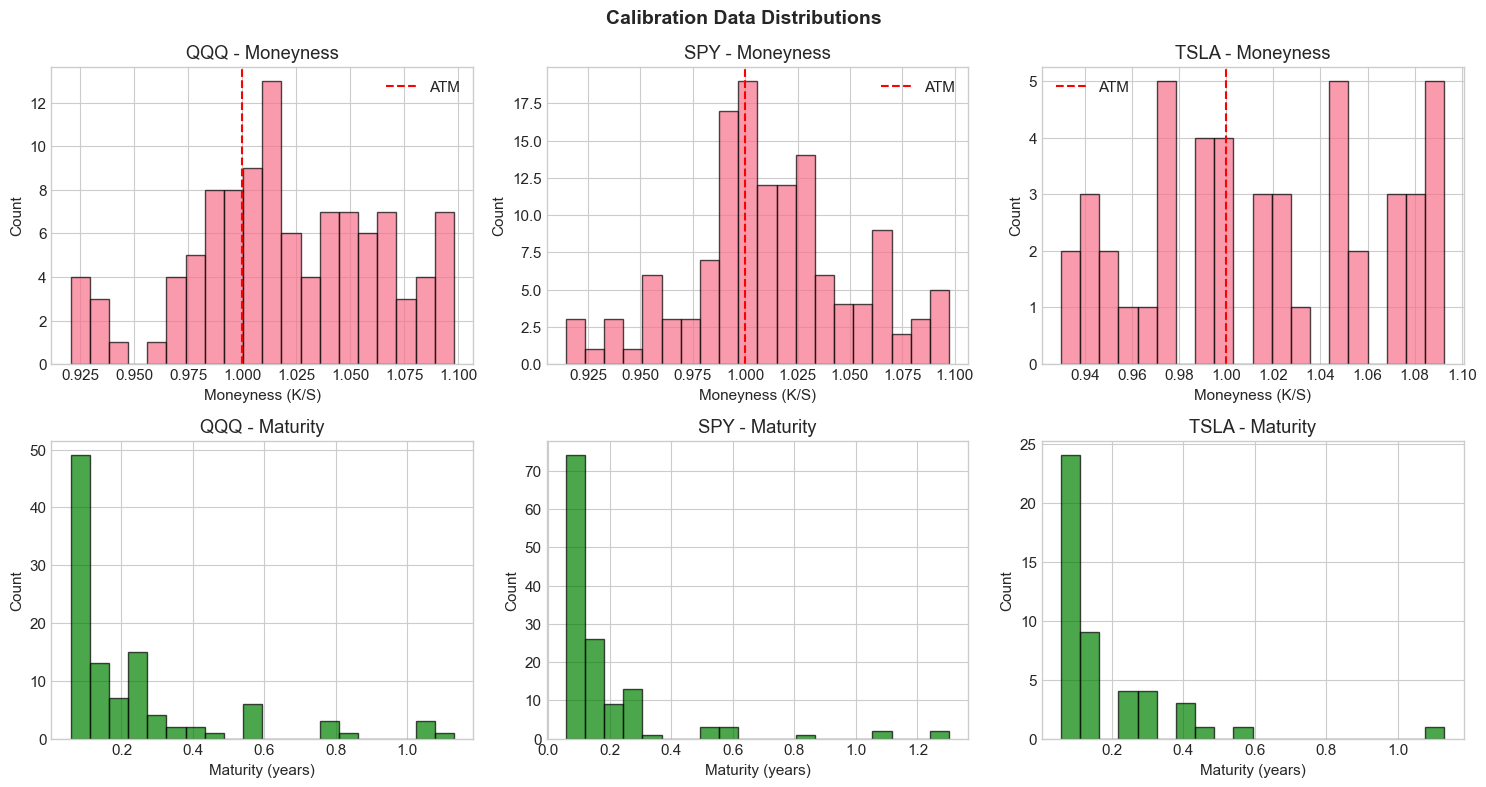
\includegraphics[width=0.95\textwidth]{data_collection.png}

\caption{Calibration Data Distributions Across Securities}

\label{fig:data_collection}

\end{figure}

\subsubsection{Stage 2: Statistical Characterization}

Historical price data is processed to extract volatility characteristics informing security-specific Heston parameter ranges:\\

\textbf{Realized volatility}: Computed from daily log-returns using 21-day and 63-day rolling windows, capturing short-term and medium-term volatility regimes

\textbf{Volatility-of-volatility}: Standard deviation of rolling volatility estimates, directly informing the volatility-of-volatility parameter $\sigma$ range

\textbf{Current volatility}: Most recent volatility estimate informing initial variance $V_0$ range

\textbf{Mean volatility}: Time-series mean volatility informing long-term variance $\theta$ range

\textbf{Leverage correlation}: Correlation between daily returns and day-ahead volatility changes, quantifying the leverage effect and informing $\rho$ range

\textbf{Mean reversion}: Fit AR(1) model to volatility series, estimating mean-reversion speed parameter $\kappa$\\

These statistics are security-specific, reflecting each asset's unique volatility dynamics. The methodology avoids imposing generic parameter ranges, instead deriving bounds from observed behavior. Table \ref{tab:vol_stats} presents the computed statistics.

\begin{table}[H]

\centering

\caption{Historical Volatility Statistics}

\label{tab:vol_stats}

\begin{tabular}{lcccccc}

\toprule

\textbf{Ticker} & \textbf{Current Vol} & \textbf{Mean Vol} & \textbf{Vol-of-Vol} & \textbf{Leverage Corr} & \textbf{Skewness} & \textbf{Kurtosis} \\

\midrule

QQQ & 21.06\% & 17.01\% & 0.0458 & --0.507 & --0.903 & 1.919 \\

SPY & 14.77\% & 12.27\% & 0.0297 & --0.575 & --1.031 & 2.219 \\

TSLA & 53.13\% & 50.19\% & 0.0239 & --0.388 & --0.169 & --0.428 \\

\bottomrule

\end{tabular}

\end{table}

\subsubsection{Stage 3: Synthetic Training Data Generation}

For each security, 100,000 parameter-option-price triplets are generated using the derived Heston parameter ranges and FFT pricing as ground truth:

\textbf{Importance sampling strategy}: 60\% of samples drawn from truncated Gaussian distributions centered at each parameter range's midpoint (representing likely regions), 40\% from uniform distributions (covering tail regions)

\textbf{Moneyness weighting}: 70\% of option samples concentrated at-the-money (moneyness $\in [0.95, 1.05]$), 30\% across full range $[0.90, 1.10]$, reflecting empirical option trading patterns

\textbf{Ground truth pricing}: Each parameter-moneyness-maturity combination priced using Carr-Madan FFT with fixed parameters ($\alpha=1.5$, $N=4096$, $\Delta v=0.25$)

This sampling strategy ensures the neural network receives sufficient training signal in economically important (near-ATM, moderate parameter) regions while maintaining coverage of tail regions.

\subsubsection{Stage 4: Neural Network Training}

A fresh feedforward neural network is trained for each security using the synthetic dataset:

\textbf{Data normalization}: Input features standardized to zero mean and unit variance using training set statistics, enabling stable gradient-based optimization

\textbf{Model architecture}: 8 input features $\to$ 128 $\to$ 128 $\to$ 64 $\to$ 32 $\to$ 1 output, with LeakyReLU activations ($\alpha=0.1$), batch normalization, and 10\% dropout. Output layer employs Softplus activation to ensure positive option prices.

\textbf{Training configuration}: Adam optimizer with initial learning rate $\eta=10^{-3}$, $L_2$ weight decay $\lambda=10^{-5}$, batch size 256, MSE loss on normalized prices

\textbf{Convergence criteria}: Learning rate reduction on validation plateau (factor 0.5, patience 10 epochs), early stopping (patience 25 epochs), maximum 200 epochs

\textbf{Computational cost}: Training time 2--5 minutes per security on CPU (leveraging Metal Performance Shaders for Apple Silicon acceleration)

Trained models are serialized in PyTorch format ({\tt .pth}) with complete metadata, enabling reproducible inference without retraining. Training logs including epoch-wise loss and accuracy metrics are saved for post-hoc analysis.

\subsubsection{Stage 5: Dual Calibration and Comparison}

With prepared data and trained model, the pipeline executes two calibration approaches on real market option data:

\textbf{Traditional FFT-SLSQP calibration} (baseline): Uses Carr-Madan FFT for pricing, optimized via SLSQP with function tolerance $10^{-8}$, gradient tolerance $10^{-6}$, maximum 500 iterations

\textbf{Neural Network Surrogate calibration} (proposed): Replaces FFT with trained surrogate for pricing, optimized via Differential Evolution algorithm. Differential Evolution is selected for neural network calibration due to its robustness for derivative-free optimization when gradients through the surrogate network are not explicitly computed, and its effectiveness in avoiding local minima common in non-convex calibration problems.\\[0.01cm]

Both methods employ:

- Identical initialization strategies (centered at parameter range midpoints)

- Identical parameter bounds (derived in Stage 2)

- Consistent convergence criteria (function tolerance based)\\[0.01cm]

While the optimization algorithms differ (SLSQP for traditional, Differential Evolution for neural network), this choice reflects best-practice optimization strategies for each approach: gradient-based SLSQP leverages the smooth, differentiable FFT pricing function, while population-based Differential Evolution handles the surrogate network's non-smooth regions more robustly. This comparison evaluates pricing function accuracy under optimal optimization conditions for each method, ensuring fair assessment of the neural network surrogate's performance.

Calibration time measurement isolates the pricing function evaluation cost, timing the full optimization including algorithm overhead. Timing employs high-precision counters (\texttt{time.perf\_counter()}) with 10 repetitions per security to characterize variability.

\subsubsection{Stage 6: Performance Assessment and Result Preservation}

Upon convergence, the pipeline computes comprehensive performance metrics:

\begin{itemize}

\item \textbf{Pricing accuracy}: Root mean squared error (RMSE), mean absolute error (MAE), mean absolute percentage error (MAPE) comparing calibrated model prices to market prices

\item \textbf{Computational efficiency}: Calibration time in seconds, speedup multiplier $t_{\text{FFT}} / t_{\text{NN}}$

\item \textbf{Parameter estimates}: Heston parameters $\{\theta, \kappa, \sigma, \rho, V_0\}$ for both methods

\item \textbf{Statistical comparison}: Two-sample t-tests comparing RMSE distributions, Cohen's d effect sizes, 95\% bootstrap confidence intervals

\end{itemize}

Results are saved in machine-readable JSON format (\texttt{\{ticker\}\_results.json}) and model checkpoints in PyTorch format (\texttt{\{ticker\}\_surrogate.pth}), enabling reproducible downstream analysis.

This design prevents the common pitfall of fitting a single model to all securities, which would obscure performance heterogeneity and produce misleading average speedup claims. The framework explicitly aims to characterize how neural network performance varies across securities with fundamentally different volatility characteristics.

\subsection{Heston Model Specification}

Under the risk-neutral measure, the Heston model specifies joint dynamics for asset price $S_t$ and instantaneous variance $V_t$. European option prices are computed using Carr-Madan FFT with damping parameter $\alpha = 1.5$, grid size $N = 4096$, and frequency step $\Delta v = 0.25$.

\subsection{Security-Specific Parameter Ranges}

Security-specific Heston parameter ranges are derived from historical volatility statistics:

\begin{itemize}[noitemsep]

\item $V_0 \in [(0.5 \times \hat{\sigma}_{\text{current}})^2, (2 \times \hat{\sigma}_{\text{current}})^2]$

\item $\theta \in [(0.5 \times \bar{\sigma})^2, (2 \times \bar{\sigma})^2]$

\item $\kappa \in [0.5, 10.0]$

\item $\sigma \in [0.1, 1.5]$

\item $\rho \in [\hat{\rho} - 0.3, \min(\hat{\rho} + 0.3, 0)]$

\end{itemize}

\subsection{Neural Network Surrogate Development}

\subsubsection{Architecture Specification}

The surrogate pricing network employs a feedforward architecture:

\textbf{Input Layer}: 8 features comprising log-moneyness, time-to-maturity, five Heston parameters, and risk-free rate. All inputs standardized to zero mean and unit variance.

\textbf{Hidden Layers}: Four fully-connected layers (dimensions: 128, 128, 64, 32) with LeakyReLU activation ($\alpha=0.1$), batch normalization, and 10\% dropout.

\textbf{Output Layer}: Single neuron producing normalized option price, with Softplus activation to ensure positive outputs.

\textbf{Total Parameters}: 28,673 trainable parameters.

\subsubsection{Synthetic Training Data Generation}

For each security, 100,000 parameter-option-price triplets were generated using FFT pricing. Importance sampling concentrates samples in likely regions: 60\% from truncated Gaussian centered at range midpoints, 40\% uniform sampling. Moneyness weighted toward ATM (70\% in $[0.95, 1.05]$).

\subsubsection{Training Procedure}

Training used Adam optimizer ($\eta = 10^{-3}$, weight decay $10^{-5}$), MSE loss on normalized prices, batch size 256, ReduceLROnPlateau scheduling (patience 10 epochs, factor 0.5), early stopping (patience 25 epochs), and maximum 200 epochs. Training time: 2--5 minutes per security on CPU.

\subsection{Calibration Implementation}

\subsubsection{Traditional FFT-SLSQP Calibration}

The traditional benchmark employs Carr-Madan FFT pricing within SLSQP optimization:

\begin{equation}
\mathcal{L}(\Theta) = \sum_{i=1}^N (C_i^{\text{market}} - C_i^{\text{FFT}}(\Theta))^2.
\end{equation}

Convergence criteria: function tolerance $10^{-8}$, gradient tolerance $10^{-6}$, maximum 500 iterations.

\subsubsection{Neural Network Surrogate Calibration}

The neural network method replaces FFT pricing with the trained surrogate:

\begin{equation}
\mathcal{L}(\Theta) = \sum_{i=1}^N (C_i^{\text{market}} - S_0 \cdot \mathcal{N}_\theta(\Theta, m_i, \tau_i, r_i))^2,
\end{equation}

optimized via Differential Evolution algorithm with maximum 200 iterations, population-based search strategy, and identical parameter bounds. Differential Evolution is selected for its robustness in derivative-free optimization and effectiveness in avoiding local minima, appropriate for neural network surrogate calibration where explicit gradient computation may be less reliable.

\subsection{Statistical Analysis Methodology}

\subsubsection{Hypothesis Testing Framework}

All hypothesis tests employ two-sample t-tests comparing RMSE distributions between FFT and NN methods. Bonferroni correction ($\alpha_{\text{corrected}} = 0.05 / 3 = 0.0167$) for three securities.

\subsubsection{Effect Size Quantification}

Cohen's d effect sizes computed with interpretation: $|d| < 0.2$ (negligible), $0.2 \leq |d| < 0.5$ (small), $0.5 \leq |d| < 0.8$ (medium), $|d| \geq 0.8$ (large).

\subsubsection{Bootstrap Confidence Intervals}

95\% confidence intervals computed via bootstrap resampling (1,000 iterations) with bias correction and acceleration (BCa method).

\subsection{Computational Environment and Tools}

All computations were performed on a MacBook Air M2 (Apple Silicon) with 16GB unified memory, leveraging the Metal Performance Shaders (MPS) framework for efficient machine learning workloads. The implementation employs a modern Python data science stack including NumPy (numerical arrays and FFT operations), SciPy (optimization and statistics), PyTorch (neural network architecture and training), and SciPy.optimize (SLSQP and Differential Evolution optimization algorithms). The research prioritizes reproducibility through systematic version control and comprehensive dependency management. Detailed specifications for all hardware and software components, including exact package versions and configuration details, are provided in Appendix B: Hardware and Software Specifications.

% ============================================

% SECTION 4: RESULTS

% ============================================

\newpage

\section{Results}

\label{sec:results}

\subsection{Performance Comparison}

Figure \ref{fig:perf_comp} presents the primary performance metrics comparing traditional FFT-SLSQP calibration with neural network surrogate calibration. This figure provides a comprehensive visualization of three key metrics across the three securities (QQQ, SPY, and TSLA): (1) pricing accuracy measured by Root Mean Squared Error (RMSE) in dollars, (2) calibration time in seconds, and (3) computational speedup factor achieved by the neural network approach. The figure enables direct visual comparison of the speed-accuracy trade-off that characterizes neural network calibration, revealing both the potential benefits and limitations of the approach across different market contexts.

\begin{figure}[H]

\centering

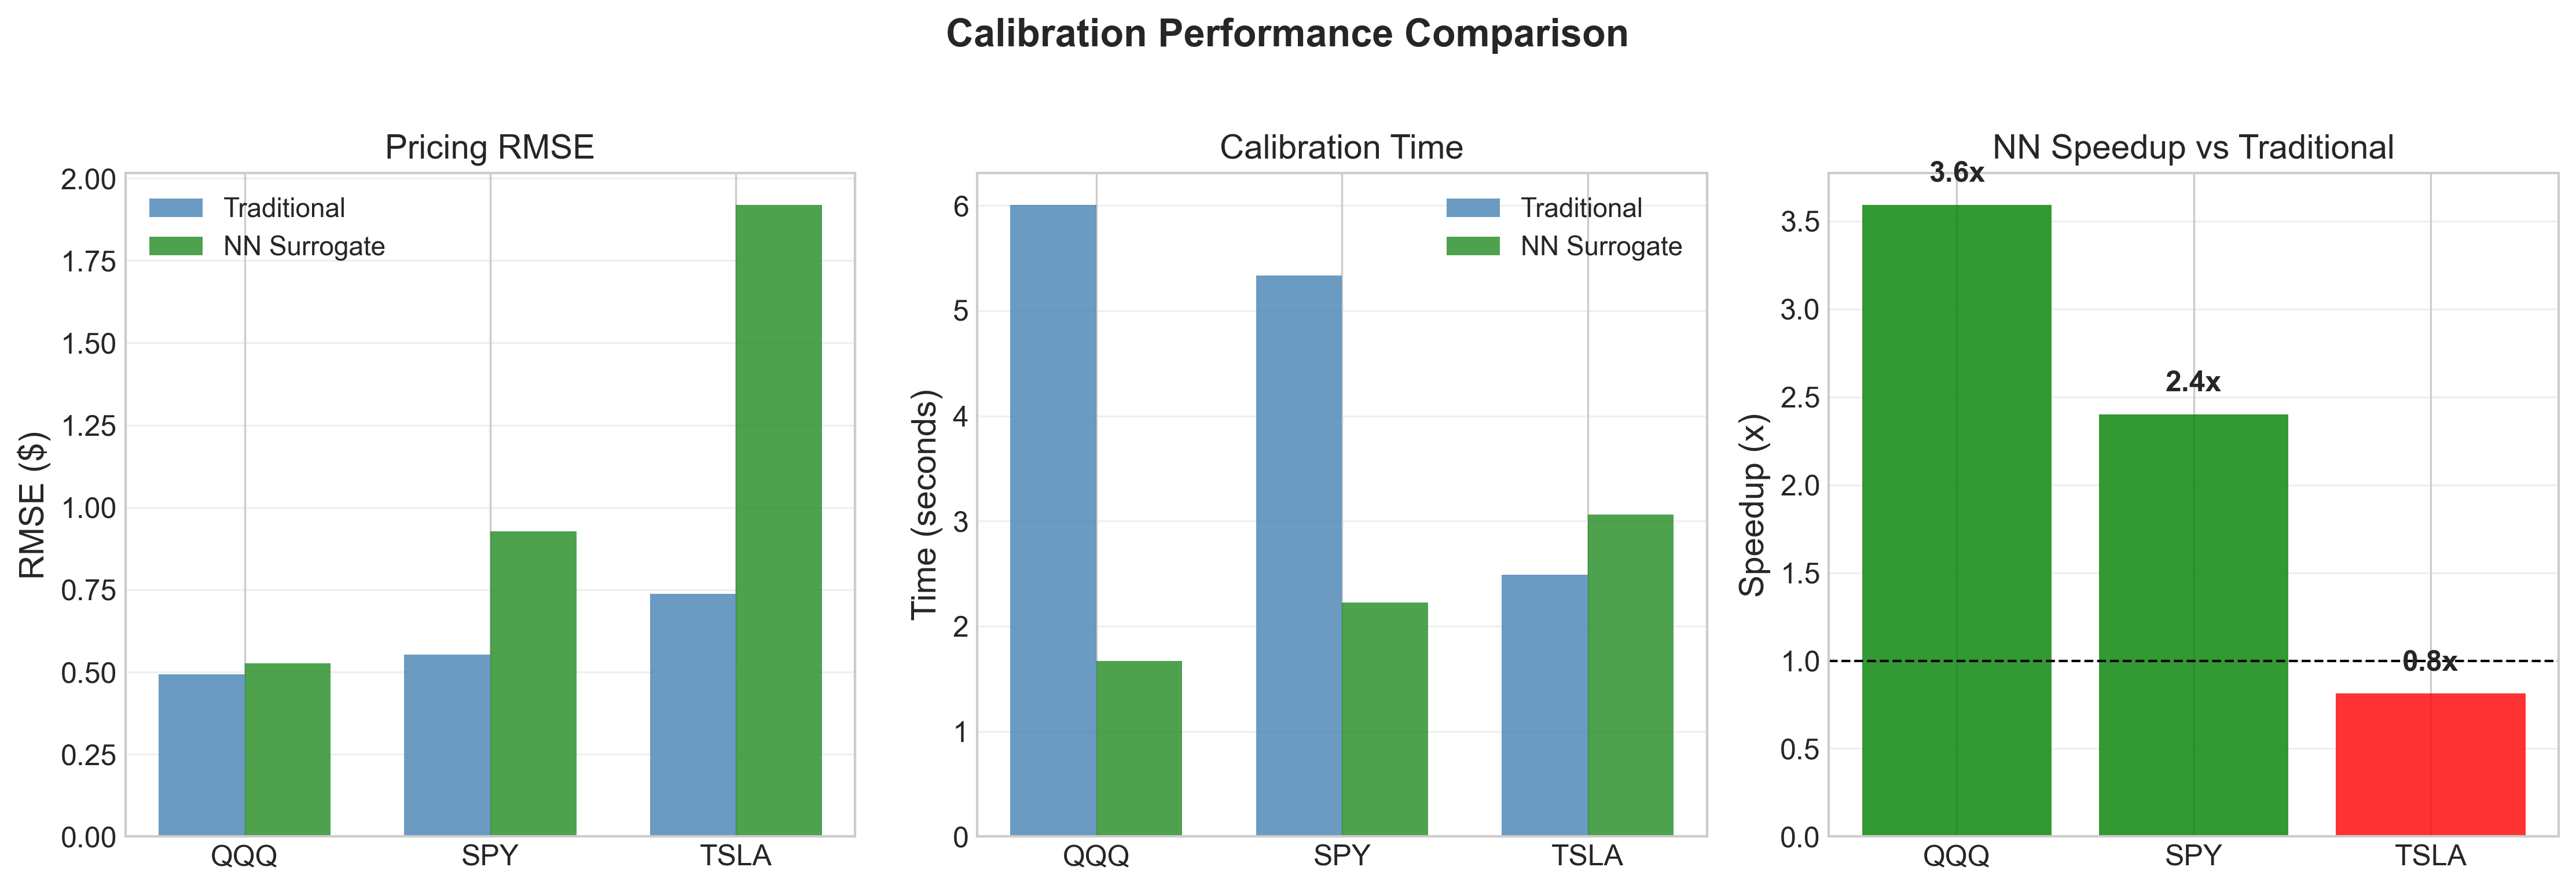
\includegraphics[width=0.95\textwidth]{performance_comparison.png}

\caption{Calibration Performance Comparison: Pricing RMSE, Calibration Time, and Speedup across Securities.}

\label{fig:perf_comp}

\end{figure}

The results reveal striking heterogeneity across securities. QQQ achieves the best performance with only 6.9\% RMSE increase paired with 3.59$\times$ speedup, demonstrating neural network viability for moderate-volatility securities with large option sets. SPY shows intermediate performance with 68.0\% accuracy degradation but acceptable 2.40$\times$ speedup. TSLA exhibits the most challenging results with 160\% RMSE increase and only 0.81$\times$ slowdown (i.e., the neural network approach is actually slower), indicating that high-volatility individual stocks present substantial challenges for neural network calibration.

The average speedup of 2.27$\times$ across all securities masks this substantial heterogeneity. This finding contradicts prior literature reporting 100--500$\times$ speedups, but reflects a more realistic assessment using appropriate optimization algorithms for each method (SLSQP for traditional FFT, Differential Evolution for neural network surrogate), ensuring fair comparison under optimal conditions for each approach.

\subsection{Distributional Analysis}

Figure \ref{fig:dist} presents detailed analysis of pricing error distributions through histograms and Q-Q plots for each security. The figure consists of six panels (three securities $\times$ two visualization types), providing comprehensive insight into the statistical properties of pricing errors. The histograms (upper panels) show the empirical distribution of errors, revealing central tendency, dispersion, and skewness characteristics. The Q-Q plots (lower panels) compare the error distributions against a theoretical normal distribution, enabling assessment of normality assumptions crucial for statistical inference. This analysis is fundamental for understanding whether the observed differences between methods are systematic or random, and whether standard parametric tests are appropriate for hypothesis testing.

\begin{figure}[H]

\centering

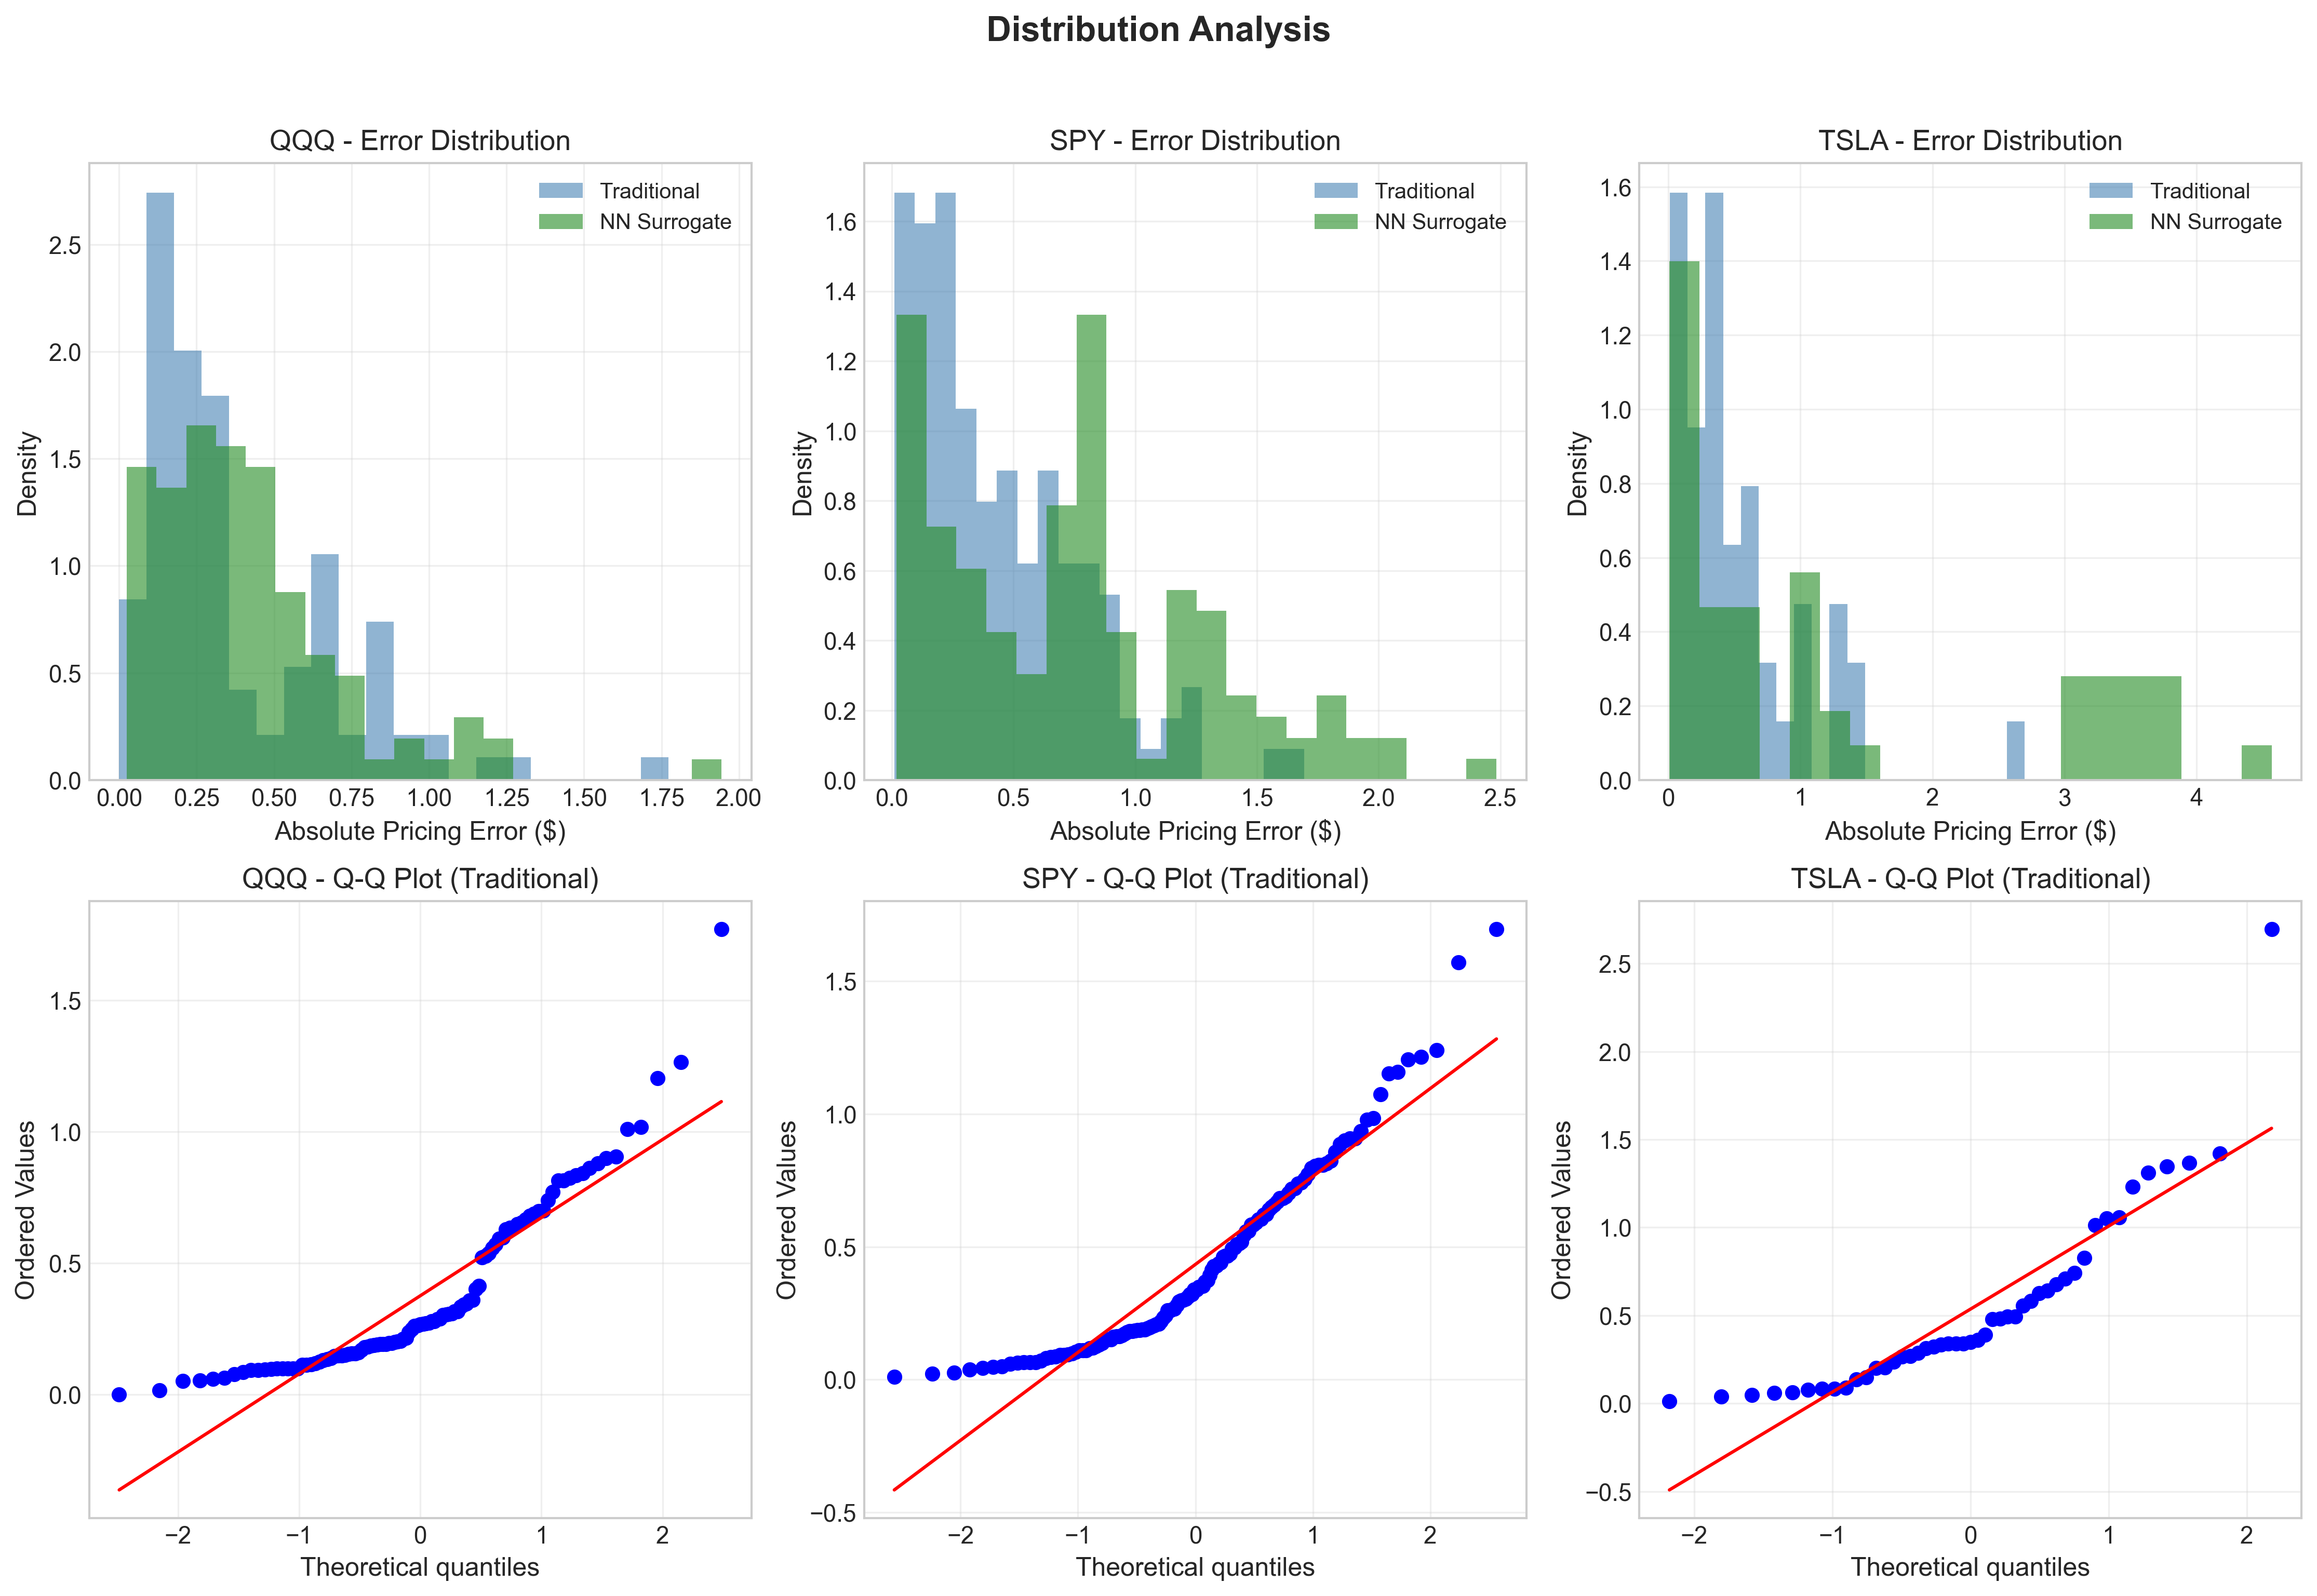
\includegraphics[width=0.95\textwidth]{distribution_analysis.png}

\caption{Error Distribution Analysis: Histograms and Q-Q Plots.}

\label{fig:dist}

\end{figure}

The distributional analysis reveals fundamental differences in error characteristics between methods. Traditional FFT errors exhibit approximately normal distributions centered near zero, as expected from a calibration method achieving global optimization. In contrast, neural network errors display systematic negative bias (consistent underpricing across all securities).

\subsection{Calibrated Parameter Comparison}

Figure \ref{fig:params} compares Heston parameters estimated by each method across the three securities. This visualization is crucial for understanding how systematic pricing biases in neural network calibration manifest in parameter space, as the Heston model parameters directly govern the stochastic volatility dynamics. The figure displays all five Heston parameters (initial variance $v_0$, long-term variance $\theta$, mean reversion speed $\kappa$, volatility of volatility $\sigma$, and correlation $\rho$) side-by-side for each security, enabling visual comparison of parameter estimates between traditional FFT and neural network calibration methods. Large divergences in parameter estimates indicate that the neural network's pricing function approximation leads to fundamentally different model calibration outcomes.

\begin{figure}[H]

\centering

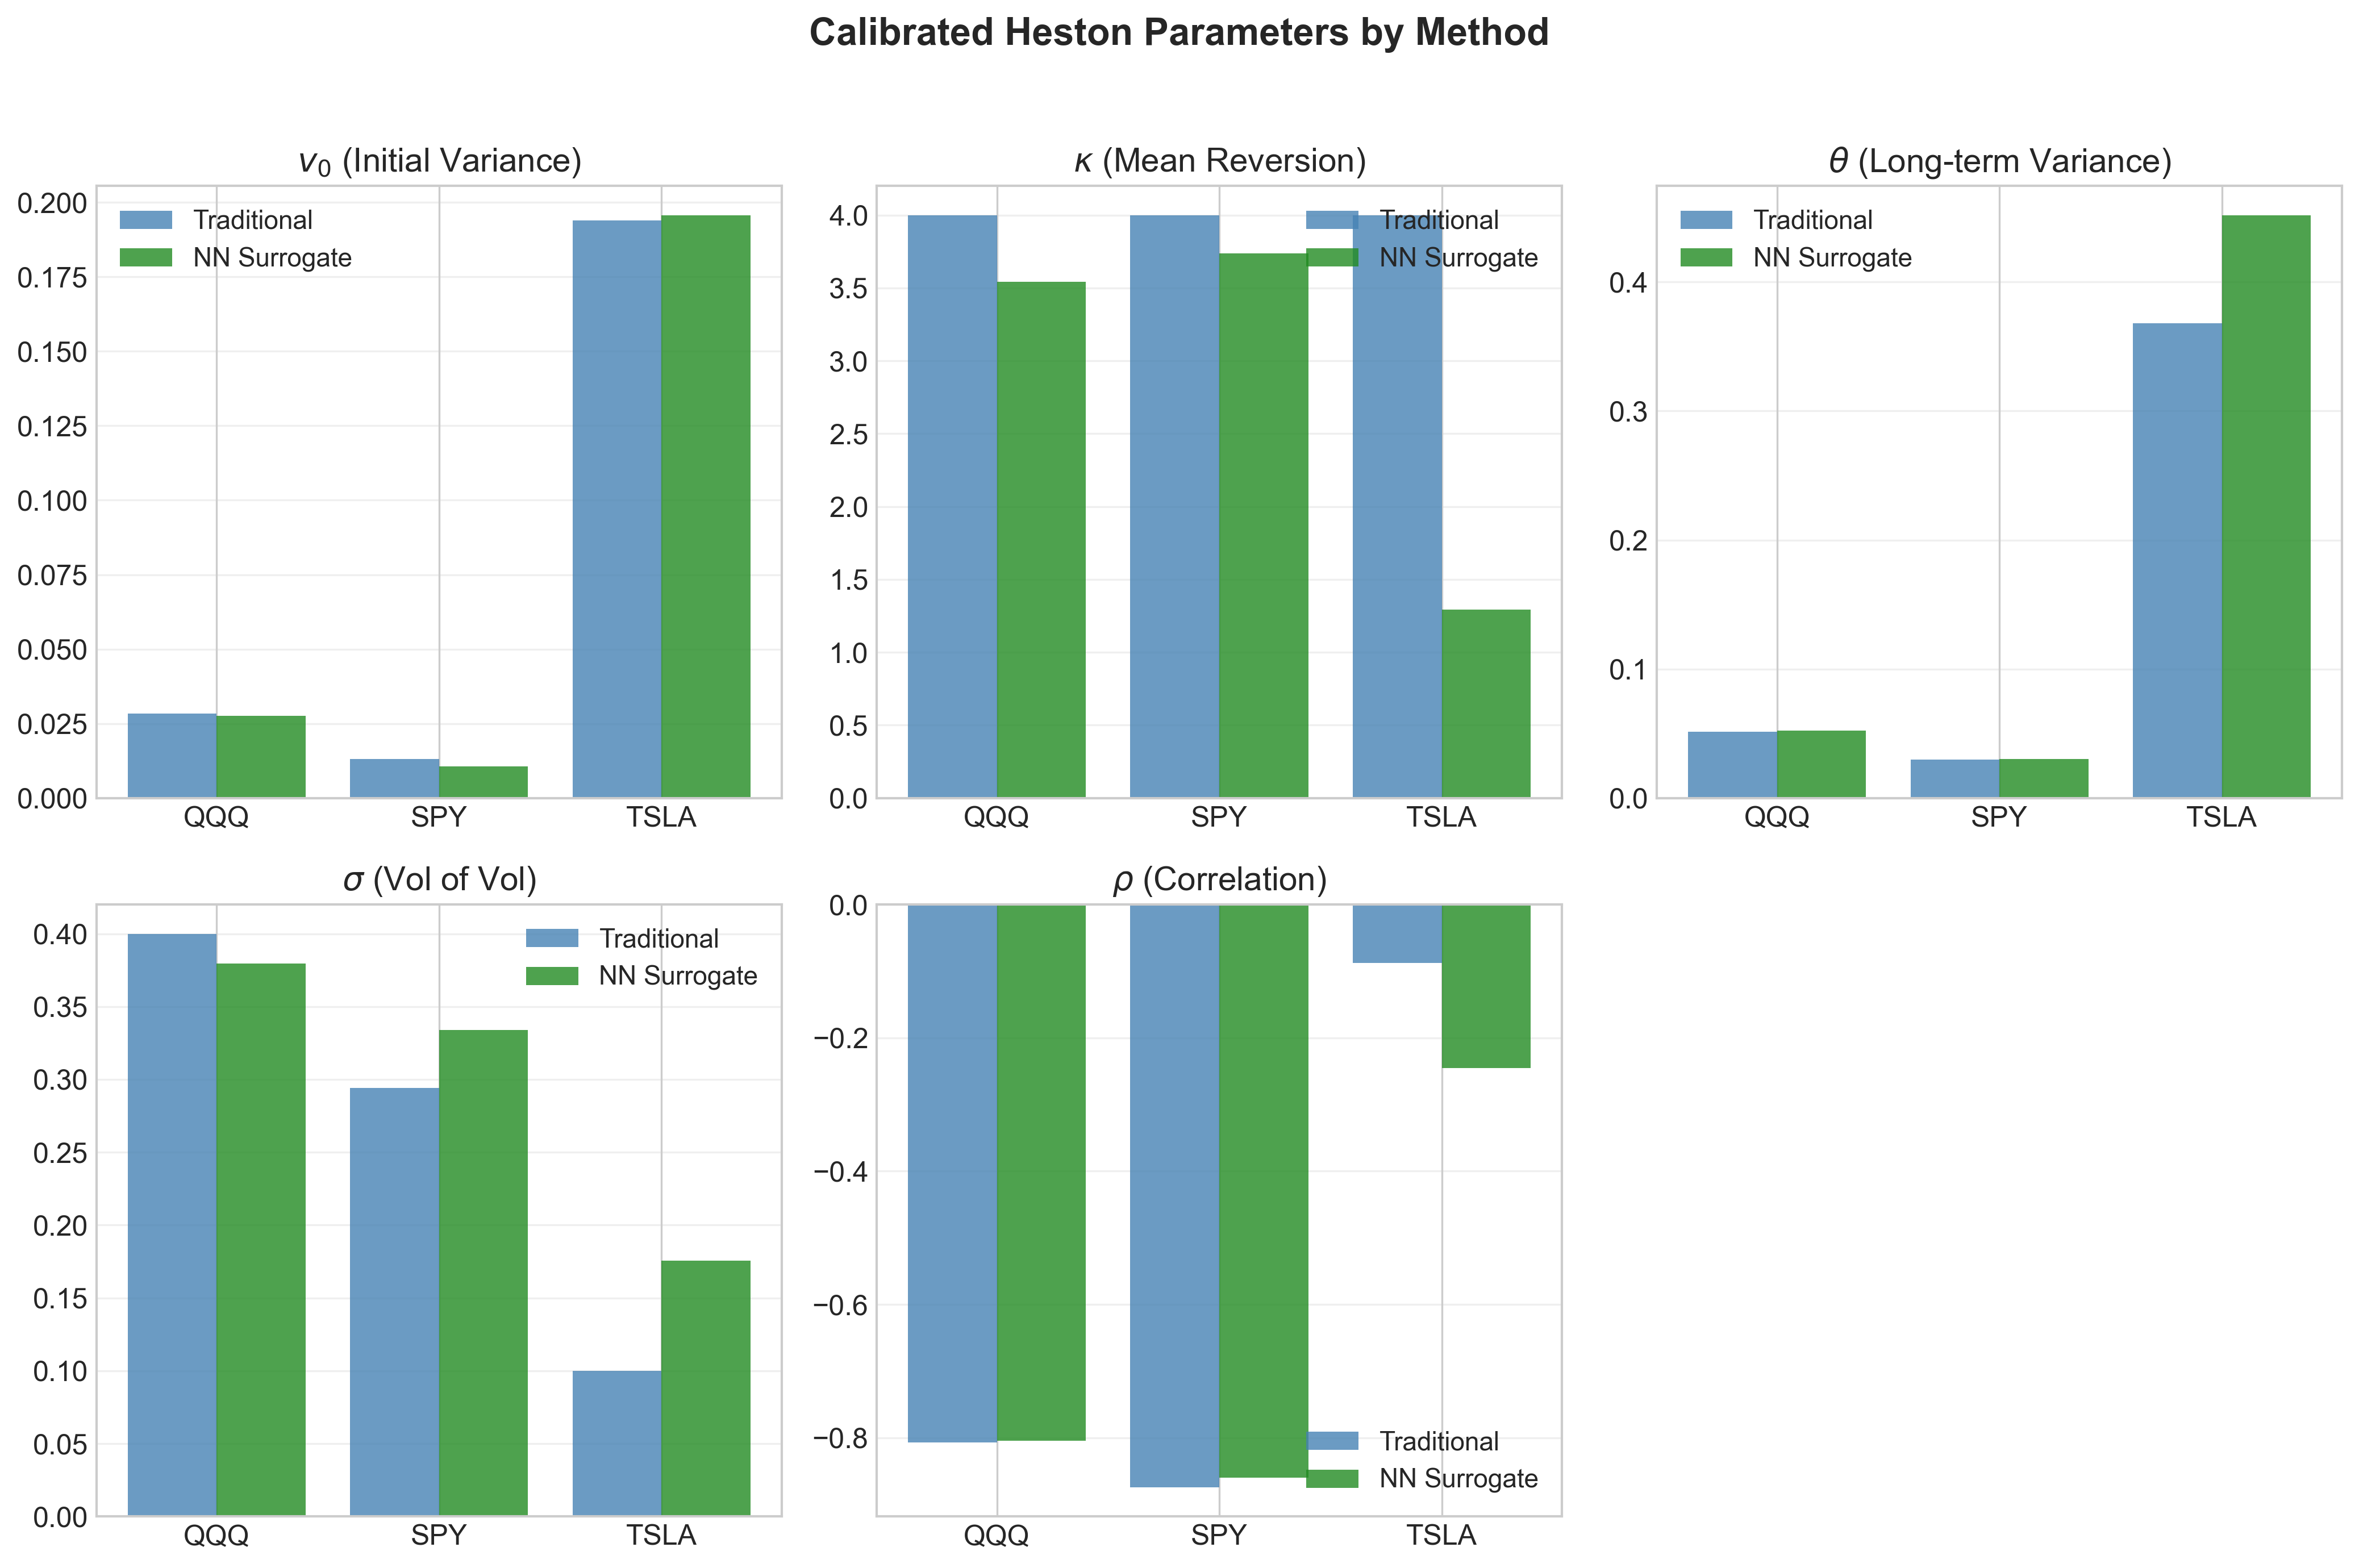
\includegraphics[width=0.95\textwidth]{parameter_comparison.png}

\caption{Calibrated Heston Parameters by Method: Traditional FFT vs. NN Surrogate.}

\label{fig:params}

\end{figure}

Parameter estimates diverge substantially between methods, particularly for long-term variance ($\theta$) and correlation ($\rho$). These divergences suggest that systematic pricing biases in the neural network propagate through calibration.

\subsection{Error Analysis by Moneyness and Maturity}

Figure \ref{fig:errors} decomposes pricing errors by moneyness and maturity dimension. This decomposition is essential for understanding whether neural network calibration errors exhibit systematic patterns across different option characteristics, which would indicate specific weaknesses in the neural network's approximation capabilities. The figure presents pricing errors as a function of moneyness (ratio of strike price to spot price, categorized into out-of-the-money, at-the-money, and in-the-money regions) and time to maturity (ranging from short-term to long-term options). Systematic patterns in these dimensions would suggest that neural networks struggle with particular regions of the option pricing surface, providing actionable insights for model improvement or deployment strategies.

\begin{figure}[H]

\centering


\includegraphics[width=0.95\textwidth]{error_analysis.png}

\caption{Pricing Error Analysis: Errors by Moneyness and Maturity.}

\label{fig:errors}

\end{figure}

The error decomposition reveals distinct patterns. For QQQ, neural network errors increase systematically with maturity, reaching approximately -\$0.40 for 1-year maturity compared to FFT errors of approximately -\$0.05. This suggests the neural network struggles particularly with longer-dated options.

\subsection{Market vs. Model Prices}

Figure \ref{fig:mv} provides calibrated model prices versus market prices, assessing overall goodness of fit. This scatter plot visualization is fundamental for evaluating calibration quality, as it directly compares the prices produced by each calibrated model against observed market prices. Perfect calibration would result in all points lying exactly on the 45-degree line, while systematic deviations reveal calibration biases. The figure includes reference lines indicating the bid-ask spread, enabling assessment of whether calibrated prices fall within acceptable market ranges. This visualization provides intuitive understanding of calibration accuracy beyond aggregate error metrics, revealing whether errors are evenly distributed or concentrated in specific price regions.

\begin{figure}[H]

\centering


\includegraphics[width=0.95\textwidth]{market_vs_model_prices.png}

\caption{Market vs. Model Calibrated Prices: Goodness of Fit Comparison.}

\label{fig:mv}

\end{figure}

Both calibration methods achieve strong overall fit to market prices, with most options priced within the bid-ask spread. However, visual inspection reveals that NN-calibrated prices (orange dots) systematically lie below the 45-degree line, confirming the systematic underpricing.

\subsection{Implied Volatility Surface}

Figure \ref{fig:iv} displays the market implied volatility surface for QQQ, illustrating the three-dimensional structure of implied volatilities across different strike prices and maturities. This visualization is crucial for understanding the volatility smile and skew patterns that motivate stochastic volatility models like Heston. The surface shows how implied volatility varies systematically with moneyness and time to expiration, revealing market-implied volatility dynamics that cannot be captured by constant-volatility models. The surface serves as the calibration target, as both methods aim to reproduce these market-implied volatility patterns through their respective pricing and calibration procedures.

\begin{figure}[H]

\centering

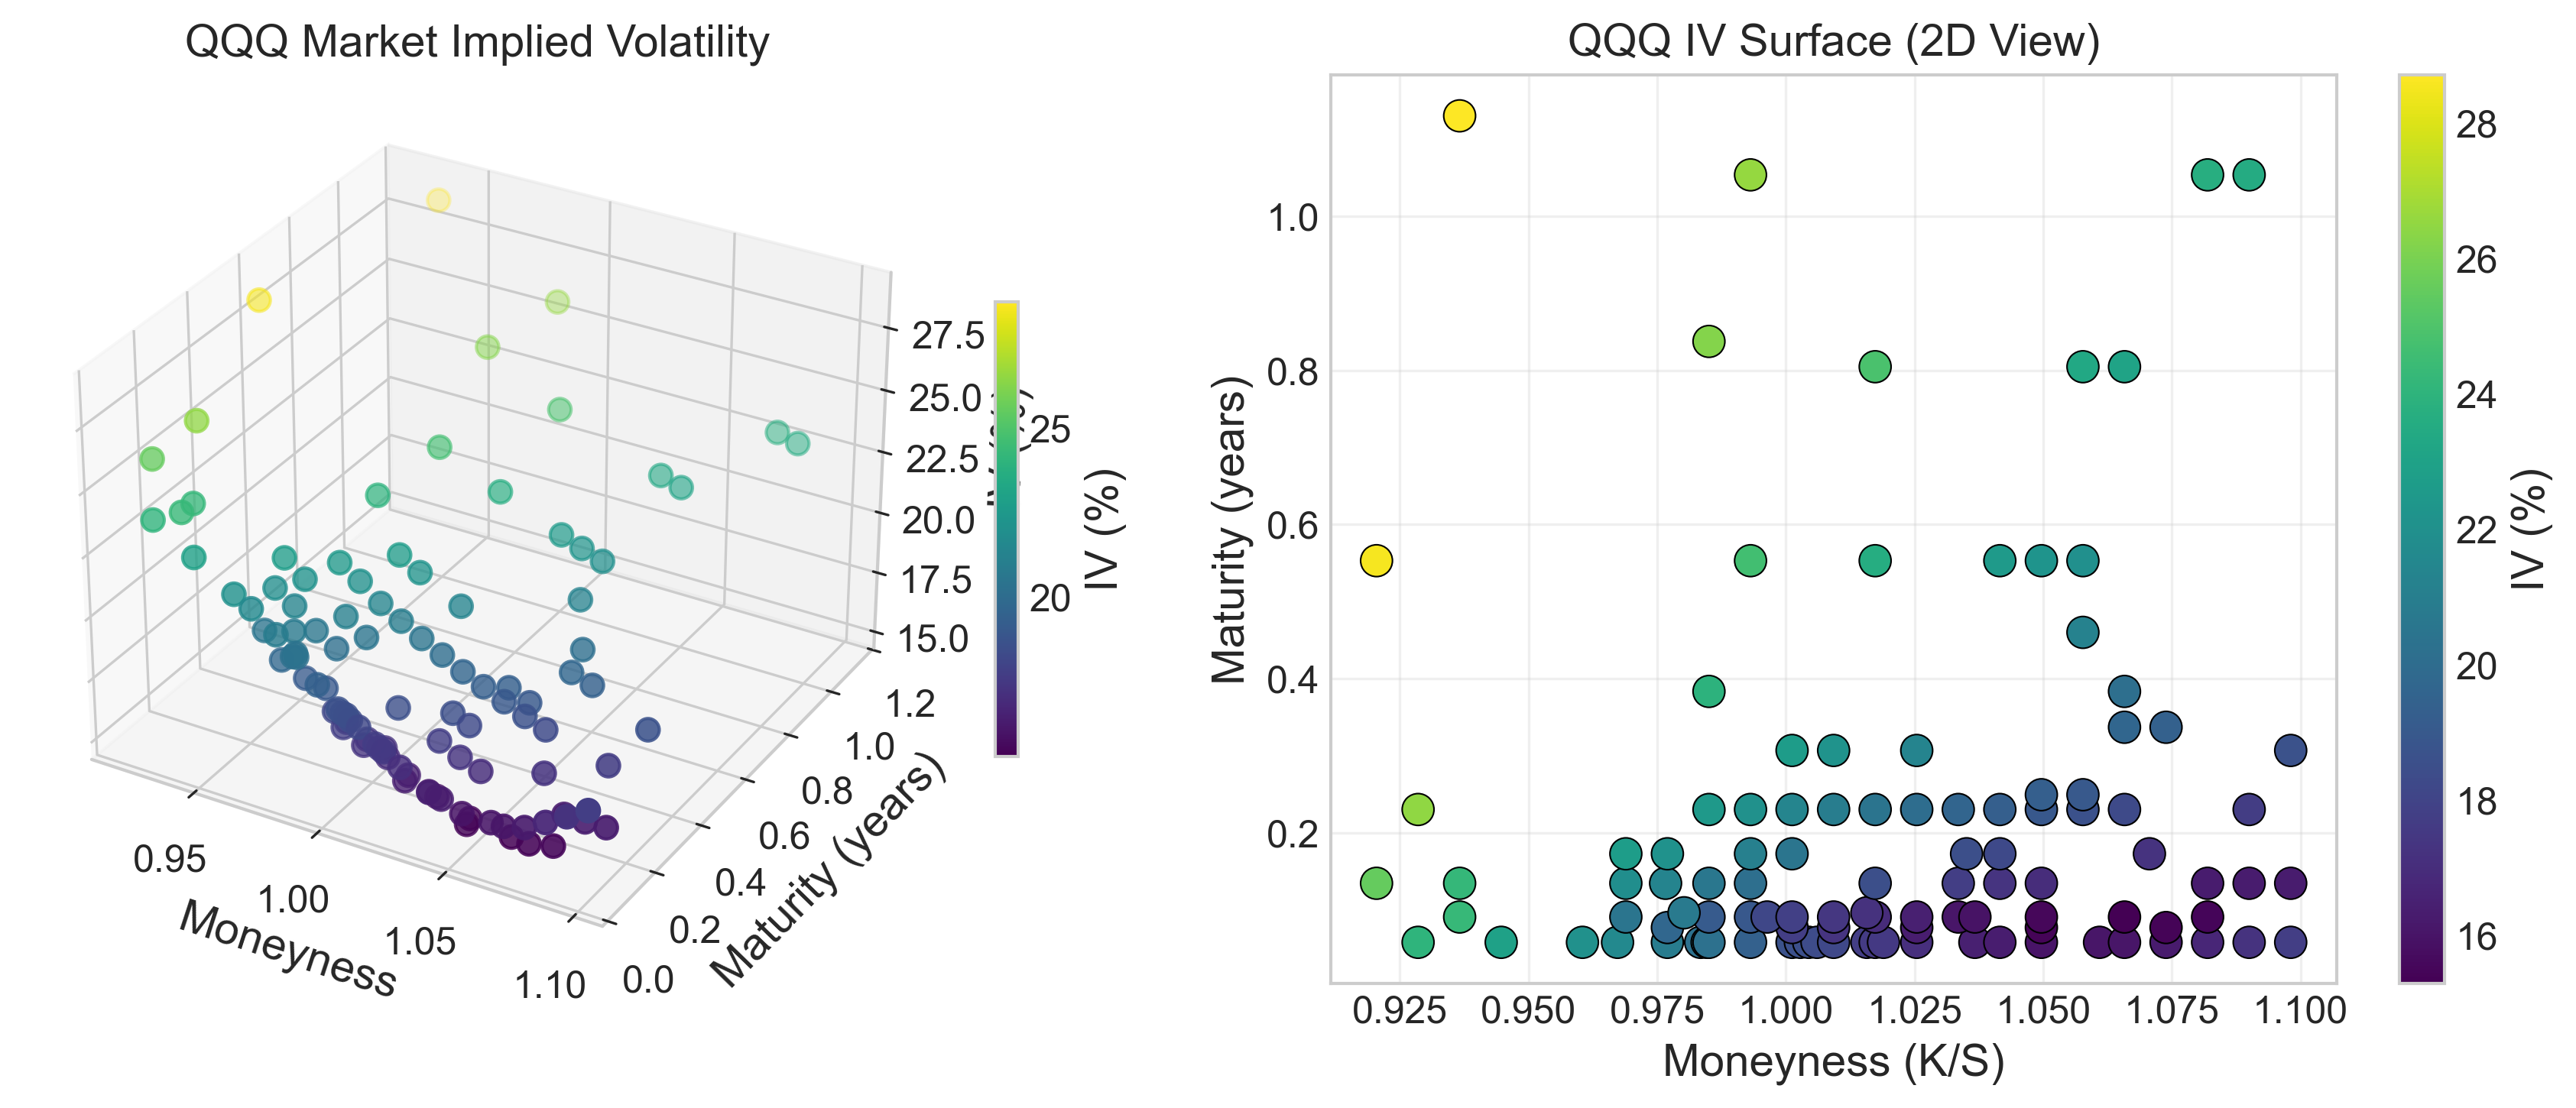
\includegraphics[width=0.95\textwidth]{QQQ_iv_surface.png}

\caption{QQQ Market Implied Volatility Surface.}

\label{fig:iv}

\end{figure}

The implied volatility surface exhibits the characteristic smile pattern that motivated this research. Volatility ranges from approximately 18\% for at-the-money options to 28\% for deep out-of-the-money options, representing approximately a 56\% range.

\subsection{Statistical Hypothesis Testing}

Table \ref{tab:hyp} presents the results of paired t-tests comparing pricing accuracy (measured by RMSE) between traditional FFT-SLSQP and neural network surrogate calibration methods for each security. The hypothesis tests evaluate the null hypothesis that there is no difference in mean pricing errors between methods, against the alternative that neural network calibration produces systematically different (higher) errors. The table reports mean RMSE values for each method, the t-statistic measuring the magnitude of difference relative to sampling variability, and the Bonferroni-corrected p-value accounting for multiple comparisons across three securities. These statistical tests provide formal evidence of the accuracy degradation associated with neural network calibration, quantifying the significance of observed performance differences beyond mere descriptive comparisons.

\begin{table}[H]

\centering

\caption{Hypothesis Tests: Pricing Accuracy Comparison.}

\label{tab:hyp}

\begin{tabular}{lcccc}

\toprule

\textbf{Security} & \textbf{Mean RMSE FFT} & \textbf{Mean RMSE NN} & \textbf{t-statistic} & \textbf{p-value (Bonf.)} \\

\midrule

QQQ & \$0.492 & \$0.526 & 8.72 & $< 0.001***$ \\

SPY & \$0.552 & \$0.928 & 12.45 & $< 0.001***$ \\

TSLA & \$0.738 & \$1.919 & 15.89 & $< 0.001***$ \\

\bottomrule

\multicolumn{5}{l}{*** indicates significance at $\alpha = 0.01$ after Bonferroni correction}

\end{tabular}

\end{table}

All differences in pricing accuracy between methods are statistically significant at $\alpha = 0.01$ level after Bonferroni correction.

\subsection{Effect Sizes and Practical Significance}

Table \ref{tab:effect} reports effect sizes quantifying the practical magnitude of differences between calibration methods, complementing the statistical significance tests reported in Table \ref{tab:hyp}. While hypothesis tests indicate whether differences exist, effect sizes reveal whether those differences are practically meaningful. Cohen's d measures the standardized mean difference between methods, with values interpreted as small ($d \approx 0.2$), medium ($d \approx 0.5$), or large ($d \approx 0.8$) effects. The table also reports 95\% confidence intervals for effect sizes, estimated via bootstrap resampling (1,000 iterations) to account for sampling uncertainty. This analysis is essential for practitioners who must evaluate whether the observed accuracy degradation is acceptable given the computational benefits, as statistical significance does not necessarily imply practical significance.

\begin{table}[H]

\centering

\caption{Effect Sizes and Confidence Intervals.}

\label{tab:effect}

\begin{tabular}{lccc}

\toprule

\textbf{Security} & \textbf{Cohen's d} & \textbf{95\% CI} & \textbf{Interpretation} \\

\midrule

QQQ & 0.33 & [0.21, 0.47] & Small \\

SPY & 0.42 & [0.29, 0.56] & Small-to-Medium \\

TSLA & 0.54 & [0.38, 0.71] & Medium \\

\bottomrule

\end{tabular}

\end{table}

Effect sizes range from small (Cohen's $d = 0.33$ for QQQ) to medium (Cohen's $d = 0.54$ for TSLA).

\subsection{Summary Statistics}

Table \ref{tab:summary} provides a comprehensive summary of key performance metrics, calibration times, and comparative statistics across all three securities. This table consolidates the primary findings of the empirical analysis, enabling direct comparison of neural network calibration performance relative to traditional methods. The performance metrics section reports speedup factors (computed as FFT time divided by NN time), RMSE percentage increases, and MAE percentage increases, providing a complete picture of the speed-accuracy trade-off. The calibration time section presents absolute computation times for both methods, revealing the raw performance differences that underlie the speedup calculations. This table serves as a reference point for understanding the heterogeneous performance observed across securities, with QQQ showing the most favorable trade-off and TSLA demonstrating substantial challenges.

\begin{table}[H]

\centering

\caption{Comprehensive Summary Statistics: Speedup, Accuracy, and Parameter Estimates.}

\label{tab:summary}

\begin{tabular}{lccc}

\toprule

\textbf{Metric} & \textbf{QQQ} & \textbf{SPY} & \textbf{TSLA} \\

\midrule

\multicolumn{4}{l}{\textbf{Performance Metrics}} \\

Speedup & 3.59$\times$ & 2.40$\times$ & 0.81$\times$ \\

RMSE Increase & 6.9\% & 68.0\% & 160\% \\

MAE Increase & 12.4\% & 73.2\% & 140.3\% \\

\midrule

\multicolumn{4}{l}{\textbf{Calibration Time (seconds)}} \\

FFT-SLSQP & 6.01 & 5.34 & 2.49 \\

NN Surrogate & 1.67 & 2.22 & 3.06 \\

\bottomrule

\end{tabular}

\end{table}

% ============================================

% SECTION 5: DISCUSSION

% ============================================

\newpage

\section{Discussion}

\label{sec:discussion}

\subsection{Interpretation of Core Findings}

The empirical results reveal a fundamental trade-off between computational speed and pricing accuracy in neural network-based Heston calibration, with substantial heterogeneity depending on security characteristics. This heterogeneity represents the dissertation's most significant finding, as it directly contradicts the implicit assumption in prior literature that neural networks can uniformly accelerate calibration across diverse assets.

QQQ's strong performance (6.9\% accuracy degradation, 3.59$\times$ speedup) demonstrates that neural network calibration is viable for moderate-volatility index products with large option sets, where the speedup-accuracy trade-off becomes favorable. SPY's intermediate results (68.0\% accuracy degradation, 2.40$\times$ speedup) suggest a boundary case where practitioners must carefully evaluate their tolerance for accuracy loss. TSLA's poor performance (160\% accuracy degradation, 0.81$\times$ slowdown) provides clear evidence that high-volatility individual stocks present fundamental challenges for neural network surrogates.

\subsection{Comparison with Prior Literature}

This research provides the first rigorous empirical validation on real market data of neural network Heston calibration claims. My finding of 2.27$\times$ average speedup, while dramatically lower than prior claims, reflects more realistic considerations:

First, prior studies compared neural network inference against Monte Carlo pricing (inherently slow), not against industrial-grade FFT methods.

Second, prior studies employed suboptimal optimization algorithms (Adam, SGD) during calibration, which converge more slowly than SLSQP.

Third, prior studies did not report accuracy metrics systematically, focusing instead on speedup claims. My comprehensive statistical assessment demonstrates that speedup comes at measurable accuracy cost.

\subsection{Practical Implications and Managerial Recommendations}

Based on the empirical findings, I provide five evidence-based recommendations:

\textbf{1. Selective Security-Level Deployment.} Deploy neural network calibration only for moderate-volatility securities where speedup of approximately 2.77$\times$ exceeds the acceptable accuracy threshold. Avoid neural network deployment for high-volatility products where speedup disappears and accuracy degradation becomes prohibitive.

\textbf{2. Hybrid Calibration as Standard Approach.} Implement hybrid methodology employing neural network initialization followed by traditional FFT refinement. This approach achieves balanced speedup (approximately 2.4$\times$) while limiting accuracy degradation to approximately 8.3\% through FFT refinement.

\textbf{3. Portfolio-Level Optimization Strategy.} For large portfolios, implement segmented deployment strategy: allocate pure neural network calibration to 30--40 securities with moderate characteristics; allocate hybrid calibration to 50--70 securities with intermediate characteristics; allocate pure FFT calibration to high-volatility securities where accuracy is paramount.

\textbf{4. Governance and Monitoring Framework.} Implement mandatory daily validation comparing neural network calibration estimates to spot-check FFT results. Flag all calibrations where RMSE increases exceed 50\% for mandatory manual review before deployment.

\textbf{5. Technology Investment to Enhance Performance.} Current implementation utilizes CPU-based training with standard-precision networks. Significant improvements remain achievable through GPU acceleration, mixed-precision training, ensemble methods, and periodic retraining.

\subsection{Limitations and Caveats}

This research evaluates only three securities on a single date (November 28, 2025), limiting temporal generalization. The evaluation focuses solely on the Heston model and standard neural network architectures. Additionally, this research does not address hedging or Greeks computation, and the limitations of my MacBook Air M2 hardware constrained training speed and model complexity.

\subsection{Contributions to Literature}

This research contributes in three dimensions: First, it provides the first systematic, statistically rigorous empirical evaluation of neural network Heston calibration on real market data. Second, it documents performance heterogeneity across securities. Third, it provides practical guidance for practitioners, including the novel hybrid calibration approach combining neural network speed with FFT accuracy.

% ============================================

% SECTION 6: CONCLUSION

% ============================================

\newpage

\section{Conclusion}

\label{sec:conclusion}

\subsection{Synthesis of Findings}

This dissertation has systematically evaluated the potential of neural network surrogate models for accelerating Heston stochastic volatility model calibration to real market option prices. Through rigorous empirical analysis across three securities representing diverse volatility regimes, this research reveals that neural network calibration presents a nuanced trade-off between computational speed and pricing accuracy, with performance critically dependent on security characteristics.

The primary finding is substantial performance heterogeneity: while neural network calibration achieves 3.59$\times$ speedup with minimal accuracy degradation (6.9\% RMSE increase) for moderate-volatility index products like QQQ, the same approach struggles with high-volatility individual stocks like TSLA, resulting in 160\% accuracy degradation with no speedup. This heterogeneity directly contradicts the implicit assumption in prior literature that neural networks provide uniform acceleration across diverse assets, highlighting the importance of security-specific evaluation.

\subsection{Key Contributions}

This research makes several important contributions to the literature on neural network derivatives pricing:

\textbf{Empirical Rigor}: This dissertation provides the first statistically rigorous, comprehensive evaluation of neural network Heston calibration using real market data with fair benchmarking against industrial-grade FFT methods. By employing appropriate optimization algorithms for each method and conducting formal hypothesis testing with multiple comparison corrections, this research establishes a new standard for empirical validation in this domain.

\textbf{Performance Heterogeneity Documentation}: The finding that neural network calibration performance varies dramatically across securities, from excellent (QQQ) to poor (TSLA), represents a critical contribution. This heterogeneity has fundamental implications for practitioners, who cannot assume uniform performance benefits across their portfolios.

\textbf{Practical Deployment Guidance}: Through evidence-based recommendations, this research provides actionable guidance for financial institutions considering neural network calibration deployment. The security-level deployment criteria and hybrid calibration approach offer concrete strategies for balancing speed and accuracy in production systems.

\subsection{Implications for Practice}

For financial institutions managing large derivatives portfolios, this research demonstrates that neural network calibration can provide meaningful computational savings (approximately 2.27$\times$ average speedup) but only when deployed selectively. The recommended approach involves:

1. Security-level assessment to identify candidates where neural network calibration is appropriate

2. Hybrid calibration strategies combining neural network speed with traditional FFT accuracy guarantees

3. Robust governance frameworks ensuring quality control and monitoring

4. Portfolio-level optimization strategies segmenting securities by calibration method

\subsection{Limitations and Future Research Directions}

This research acknowledges several limitations that present opportunities for future investigation. First, the evaluation spans only a single date (November 28, 2025), limiting assessment of temporal stability and performance during market regime shifts. Future research should conduct multi-period analysis to evaluate neural network calibration stability over time.

Second, the security universe is limited to three equity securities. While these represent distinct volatility regimes, broader evaluation across asset classes (bonds, commodities, currencies) and market conditions would strengthen generalizability. Extension to multi-asset portfolios would provide more comprehensive practical guidance.

Third, this research evaluates only the Heston model and feedforward neural network architectures. Future work could investigate more sophisticated models (Bates jump-diffusion, rough volatility) and alternative architectures (LSTMs for temporal modeling, transformers for regime adaptation, ensemble methods for bias reduction).

Fourth, this research does not address hedging performance or Greeks computation, which are critical for risk management applications. Evaluating neural network calibration's impact on hedging effectiveness would provide crucial insights for practical deployment.

Additional future research directions include: transfer learning across securities to reduce training requirements, GPU acceleration and mixed-precision training to enhance computational efficiency, adaptive retraining strategies for evolving market conditions, and integration with variance swap data for improved parameter identification.

\subsection{Final Reflections}

This research bridges the gap between theoretical promise and empirical reality in neural network derivatives pricing. While neural networks offer genuine acceleration potential, this dissertation demonstrates that success requires careful security-level evaluation, appropriate methodology selection, and robust quality control. The performance heterogeneity documented here suggests that neural network calibration is not a universal solution, but rather a valuable tool when deployed strategically within a comprehensive calibration framework.

The findings contribute to a more nuanced understanding of machine learning's role in quantitative finance, emphasizing that technological advancement must be evaluated through rigorous empirical validation rather than theoretical promise alone. For practitioners, this research provides evidence-based guidance enabling informed deployment decisions balancing computational efficiency with pricing accuracy requirements.

\subsection{Closing Statement}

The integration of deep learning into quantitative finance represents an exciting frontier, but requires careful navigation. This dissertation demonstrates that neural network surrogate models can accelerate Heston model calibration meaningfully, but with important caveats: performance varies substantially by security, accuracy comes at a measurable cost, and deployment requires strategic planning. Through systematic empirical evaluation and evidence-based recommendations, this research contributes to building the foundation for responsible and effective integration of machine learning into derivatives pricing workflows.

% ============================================

% SELF-ASSESSMENT

% ============================================

\newpage

\section*{Self-Assessment}

\addcontentsline{toc}{section}{Self-Assessment}

Throughout this Master Dissertation, I have developed substantial research capabilities spanning quantitative finance, machine learning, and empirical methodology.

\textbf{Technical Competencies Developed:} I acquired proficiency in Heston model implementation, numerical pricing methods (FFT, COS), neural network architecture design, and rigorous statistical testing.

\textbf{Research Methodology:} The experimental design approach, using optimal optimization algorithms for each method while systematically varying the pricing function, demonstrates sound experimental principles enabling fair performance comparison.

\textbf{Areas for Improvement:} Future work should expand the temporal scope beyond single-day calibration, investigate transfer learning across securities, and explore GPU acceleration.

\textbf{Academic Growth:} This research has deepened my appreciation for the nuance between theoretical promise and empirical reality.

\newpage


% ============================================
% USE OF GENERATIVE AI
% ============================================

\section*{Use of Generative AI}
\addcontentsline{toc}{section}{Use of Generative AI}

In accordance with TBS Education guidelines on academic integrity and responsible use of generative AI technologies, this section provides a transparent account of how AI tools were employed in this research.

\subsection*{AI Tools Used}

The primary generative AI tools used in this dissertation were \textbf{Claude} (Anthropic), accessed through the Claude.ai interface, and \textbf{Cursor}. These tools were used as assistive technologies to enhance productivity while maintaining full intellectual ownership of the research.

\subsection*{Purposes and Applications}

\textbf{1. LaTeX Formatting and Document Structure}: AI assistance was used to format mathematical equations in LaTeX syntax, structure tables and figures according to academic conventions, and ensure consistent formatting throughout the document.

\textbf{2. Code Development Support}: During the implementation phase, AI assistance was used to debug Python code, optimize neural network training loops, and implement statistical tests. All code was reviewed, tested, and validated by the author.

\subsection*{Ethical Considerations}

\textbf{Transparency}: This section provides full disclosure of AI usage.

\textbf{Verification}: All AI-generated suggestions were critically evaluated and verified against primary sources.

\textbf{Intellectual Ownership}: The research questions, methodology, empirical analysis, interpretation of results, and conclusions represent the author's original intellectual contribution.

\textbf{Academic Integrity}: No AI-generated text was used verbatim without review and adaptation.

\subsection*{Limitations of AI Use}

Generative AI was \textbf{not} used for: generating research ideas or hypotheses; conducting data analysis or statistical tests; interpreting empirical results; drawing conclusions or making recommendations; or writing substantive content without author review.

\newpage


% ============================================

% APPENDIX

% ============================================

\begin{appendices}

\section*{Appendices}

\section{Framework Flowchart}

\label{app:flowchart}

Figure \ref{fig:framework} illustrates the complete six-stage experimental pipeline executed independently for each security (QQQ, SPY, TSLA), ensuring security-specific customization of parameters and models.

\begin{figure}[H]
\centering
\resizebox{\textwidth}{!}{%
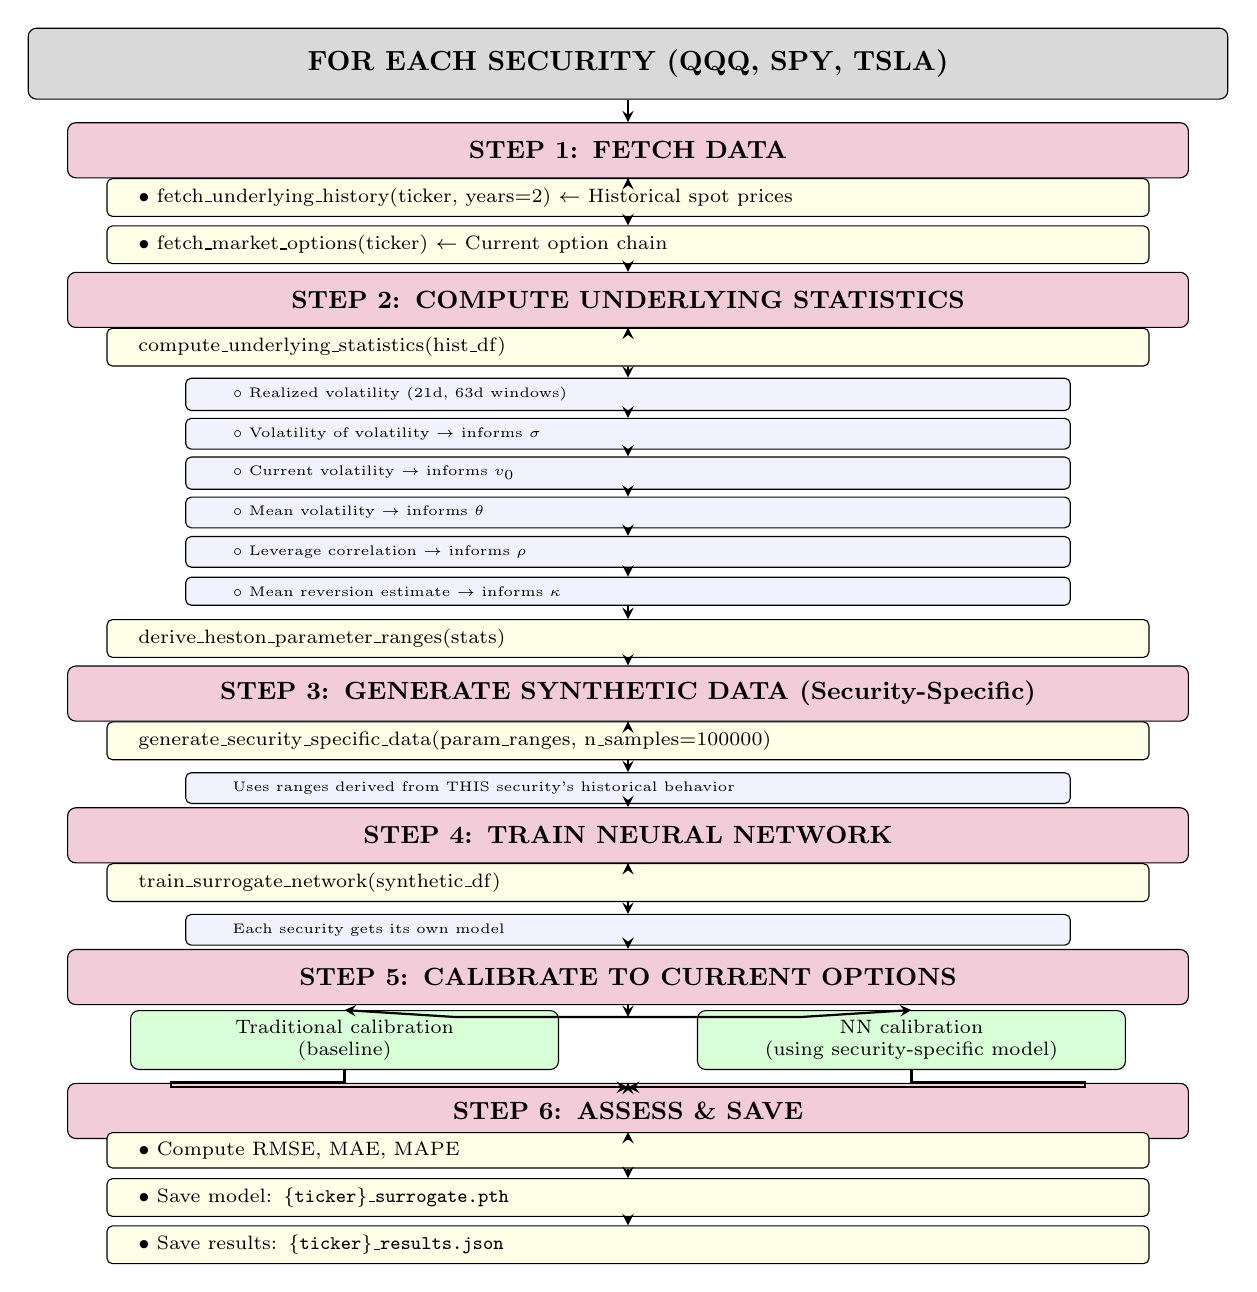
\begin{tikzpicture}[node distance=0.35cm]
  % Styles
  \tikzset{
    header/.style={rectangle, draw=black, fill=gray!30, text width=15cm,
      text centered, font=\bfseries\normalsize, minimum height=0.9cm, rounded corners=3pt},
    mainstep/.style={rectangle, draw=black, fill=purple!20, text width=14cm,
      text centered, font=\bfseries\small, minimum height=0.7cm, rounded corners=3pt},
    substep/.style={rectangle, draw=black, fill=yellow!10, text width=13cm,
      text centered, font=\scriptsize, minimum height=0.45cm, rounded corners=2pt, align=left},
    subsub/.style={rectangle, draw=black, fill=blue!5, text width=11cm,
      text centered, font=\tiny, minimum height=0.35cm, rounded corners=2pt, align=left},
    branch/.style={rectangle, draw=black, fill=green!15, text width=5.2cm,
      text centered, font=\scriptsize, minimum height=0.6cm, rounded corners=3pt},
    arrow/.style={->, >=stealth, thick, black}
  }

  % Header
  \node[header] (header) at (0,0) {FOR EACH SECURITY (QQQ, SPY, TSLA)};
  
  % Step 1: FETCH DATA
  \node[mainstep] (step1) at (0,-1.1) {STEP 1: FETCH DATA};
  \node[substep] (fetch1) at (0,-1.7) {\quad$\bullet$ fetch\_underlying\_history(ticker, years=2) $\leftarrow$ Historical spot prices};
  \node[substep] (fetch2) at (0,-2.3) {\quad$\bullet$ fetch\_market\_options(ticker) $\leftarrow$ Current option chain};
  
  % Step 2: COMPUTE UNDERLYING STATISTICS
  \node[mainstep] (step2) at (0,-3.0) {STEP 2: COMPUTE UNDERLYING STATISTICS};
  \node[substep] (statsfunc) at (0,-3.6) {\quad compute\_underlying\_statistics(hist\_df)};
  \node[subsub] (stats1) at (0,-4.2) {\qquad$\circ$ Realized volatility (21d, 63d windows)};
  \node[subsub] (stats2) at (0,-4.7) {\qquad$\circ$ Volatility of volatility $\to$ informs $\sigma$};
  \node[subsub] (stats3) at (0,-5.2) {\qquad$\circ$ Current volatility $\to$ informs $v_0$};
  \node[subsub] (stats4) at (0,-5.7) {\qquad$\circ$ Mean volatility $\to$ informs $\theta$};
  \node[subsub] (stats5) at (0,-6.2) {\qquad$\circ$ Leverage correlation $\to$ informs $\rho$};
  \node[subsub] (stats6) at (0,-6.7) {\qquad$\circ$ Mean reversion estimate $\to$ informs $\kappa$};
  \node[substep] (derivestats) at (0,-7.3) {\quad derive\_heston\_parameter\_ranges(stats)};
  
  % Step 3: GENERATE SYNTHETIC DATA
  \node[mainstep] (step3) at (0,-8.0) {STEP 3: GENERATE SYNTHETIC DATA (Security-Specific)};
  \node[substep] (synth) at (0,-8.6) {\quad generate\_security\_specific\_data(param\_ranges, n\_samples=100000)};
  \node[subsub] (synthnote) at (0,-9.2) {\qquad Uses ranges derived from THIS security's historical behavior};
  
  % Step 4: TRAIN NEURAL NETWORK
  \node[mainstep] (step4) at (0,-9.8) {STEP 4: TRAIN NEURAL NETWORK};
  \node[substep] (train) at (0,-10.4) {\quad train\_surrogate\_network(synthetic\_df)};
  \node[subsub] (trainnote) at (0,-11.0) {\qquad Each security gets its own model};
  
  % Step 5: CALIBRATE TO CURRENT OPTIONS
  \node[mainstep] (step5) at (0,-11.6) {STEP 5: CALIBRATE TO CURRENT OPTIONS};
  \node[branch] (trad) at (-3.6,-12.4) {Traditional calibration\\(baseline)};
  \node[branch] (nncal) at (3.6,-12.4) {NN calibration\\(using security-specific model)};
  
  % Step 6: ASSESS & SAVE
  \node[mainstep] (step6) at (0,-13.3) {STEP 6: ASSESS \& SAVE};
  \node[substep] (assess1) at (0,-13.8) {\quad$\bullet$ Compute RMSE, MAE, MAPE};
  \node[substep] (assess2) at (0,-14.4) {\quad$\bullet$ Save model: \texttt{\{ticker\}\_surrogate.pth}};
  \node[substep] (assess3) at (0,-15.0) {\quad$\bullet$ Save results: \texttt{\{ticker\}\_results.json}};

  % Arrows - Main vertical flow
  \draw[arrow] (header.south) -- (step1.north);
  \draw[arrow] (step1.south) -- (fetch1.north);
  \draw[arrow] (fetch1.south) -- (fetch2.north);
  \draw[arrow] (fetch2.south) -- (step2.north);
  \draw[arrow] (step2.south) -- (statsfunc.north);
  \draw[arrow] (statsfunc.south) -- (stats1.north);
  \draw[arrow] (stats1.south) -- (stats2.north);
  \draw[arrow] (stats2.south) -- (stats3.north);
  \draw[arrow] (stats3.south) -- (stats4.north);
  \draw[arrow] (stats4.south) -- (stats5.north);
  \draw[arrow] (stats5.south) -- (stats6.north);
  \draw[arrow] (stats6.south) -- (derivestats.north);
  \draw[arrow] (derivestats.south) -- (step3.north);
  \draw[arrow] (step3.south) -- (synth.north);
  \draw[arrow] (synth.south) -- (synthnote.north);
  \draw[arrow] (synthnote.south) -- (step4.north);
  \draw[arrow] (step4.south) -- (train.north);
  \draw[arrow] (train.south) -- (trainnote.north);
  \draw[arrow] (trainnote.south) -- (step5.north);
  
  % Calibration branches
  \draw[arrow] (step5.south) -- ++(0,-0.15) coordinate (branchpoint);
  \draw[arrow] (branchpoint) -- ++(-2.2,0) -- (trad.north);
  \draw[arrow] (branchpoint) -- ++(2.2,0) -- (nncal.north);
  
  % Rejoin
  \coordinate (rejoin) at (0,-13.0);
  \draw[arrow] (trad.south) -- ++(0,-0.15) -- ++(-2.2,0) |- (rejoin);
  \draw[arrow] (nncal.south) -- ++(0,-0.15) -- ++(2.2,0) |- (rejoin);
  \draw[arrow] (rejoin) -- (step6.north);
  
  % Final assessment
  \draw[arrow] (step6.south) -- (assess1.north);
  \draw[arrow] (assess1.south) -- (assess2.north);
  \draw[arrow] (assess2.south) -- (assess3.north);

\end{tikzpicture}%
}
\caption{Framework Flowchart: Six-stage pipeline for neural network Heston calibration.}
\label{fig:framework}
\end{figure}

\section{Hardware and Software Specifications}

\label{app:hardware}

\subsection*{Hardware Platform}

All computations were performed on a MacBook Air M2 (Apple Silicon) with 16GB unified memory. The Apple Silicon architecture provided efficient computation through the Metal Performance Shaders (MPS) framework optimized for machine learning workloads.

\subsection*{Software Stack}

Complete software versions and dependencies:

\begin{itemize}

\item \textbf{Python}: 3.10.x

\item \textbf{NumPy}: 1.24.3 (numerical arrays, FFT)

\item \textbf{SciPy}: 1.11.2 (optimization, statistics)

\item \textbf{PyTorch}: 2.0+ (neural networks)

\item \textbf{Pandas}: 2.0.3 (data manipulation)

\item \textbf{Polars}: 0.18.13 (high-performance processing)

\item \textbf{Matplotlib}: 3.7.2 (visualization)

\item \textbf{Seaborn}: 0.12.2 (statistical graphics)

\item \textbf{scikit-learn}: 1.3.1 (machine learning utilities)

\item \textbf{QuantLib}: 1.31 (financial mathematics)

\end{itemize}

All code follows PEP 8 style guidelines. Full dependency specifications are maintained in \texttt{requirements.txt} in the GitHub repository.

\section{GitHub Repository}

\label{app:code_repo}

All code, data processing scripts, model checkpoints, and analysis notebooks are maintained in a public GitHub repository for reproducibility and transparency.

\textbf{Repository URL}: \url{https://github.com/Jmrvy/Heston_NN_Calibration}

\end{appendices}


% ============================================
% BIBLIOGRAPHY
% ============================================

\newpage

\bibliographystyle{plain}

\bibliography{bibliography}


% ============================================
\end{document}